%
% Template for Doctoral Theses at Uppsala 
% University. The template is based on    
% the layout and typography used for      
% dissertations in the Acta Universitatis 
% Upsaliensis series                      
% Ver 5.2 - 2012-08-08                  
% Latest version available at:            
%   http://ub.uu.se/thesistemplate            
%                                         
% Support: Wolmar Nyberg Akerstrom        
% Thesis Production           
% Uppsala University Library              
% avhandling@ub.uu.se                          
%                                         
%%%%%%%%%%%%%%%%%%%%%%%%%%%%%%%%%%%%%%%%%%%

\documentclass{UUThesisTemplate}
% Nomenclature


% Package to determine wether XeTeX is used
\usepackage{ifxetex}

\ifxetex
	% XeTeX specific packages and settings
	% Language, diacritics and hyphenation
	\usepackage[babelshorthands]{polyglossia}
	\setmainlanguage{english}
	\setotherlanguages{swedish}

	% Font settings
	\setmainfont{Times New Roman}
	\setromanfont{Times New Roman}
	\setsansfont{Arial}
	\setmonofont{Courier New}
\else
	% Plain LaTeX specific packages and settings
	% Language, diacritics and hyphenation
    % Use English and Swedish languages. 
	\usepackage[swedish,english]{babel} 

	% Font settings
	\usepackage{type1cm}
	\usepackage{inputenc}
	\usepackage[T1]{fontenc}
	\usepackage{mathptmx}
	
	% Enable scaling of images on import
	\usepackage{graphicx}
\fi

% Tables
\usepackage{booktabs}
\usepackage{tabularx}

% Document links and bookmarks
\usepackage{hyperref} 

% Numbering of headings down to the subsection level
\numberingdepth{subsection}

% Including headings down to the subsection level in contents
\contentsdepth{subsection}
\setlength{\parindent}{0pt}
\usepackage{parskip}

\usepackage{biblatex}
\addbibresource{References.bib}

% Subfigures
\usepackage{caption}
\usepackage{subcaption, wrapfig, graphicx}
\usepackage[section]{placeins}

% Maths
\usepackage{amsmath,physics, esint, amssymb}
\usepackage{nicematrix}
\renewcommand{\arraystretch}{1.5} % More spacious tables
\usepackage{algorithm}
\usepackage{algpseudocodex}

% Tikz
\usepackage{tikz}
\usetikzlibrary{shapes.geometric, arrows}

% Custom defines
\newcommand{\area}{\mathrm{A}}
\newcommand{\Volume}{\mathrm{V}}
\newcommand{\nvec}{\hat{\vb{n}}}
\newcommand{\ez}{\vb{\hat{e}_z}}
\newcommand{\ex}{\vb{\hat{e}_x}}
\newcommand{\ey}{\vb{\hat{e}_y}}
\newcommand{\er}{\vb{\hat{e}_r}}
\newcommand{\ephi}{\vb{\hat{e}_\varphi}}

% Bessel functions
\newcommand{\Jn}[1]{\mathit{J}_{#1}}
\newcommand{\In}[1]{\mathit{I}_{#1}}
\newcommand{\Yn}[1]{\mathit{Y}_{#1}}

% BFF potential series
\newcommand{\Bc}{\frac{2\pi}{L}}
\newcommand{\Cnk}[1][nk]{\mathfrak{C}_{#1}}
\newcommand{\Bffok}{ \frac{1}{2}
    \sum\limits_{\substack{k=-\infty\\k\neq 0}}^\infty
    \Cnk[0,k] \In{0} \left( \Bc |k|r \right)
    \exp \left( j \Bc kz \right)
}
\newcommand{\Bffno}{ \frac{1}{2}
    \sum\limits_{\substack{n=-\infty\\n\neq 0}}^\infty
    \Cnk[n,0] r^{|n|}\exp(jn\varphi)
}
\newcommand{\Bffnk}{ \frac{1}{4}
    \sum\limits_{\substack{n=-\infty\\n\neq 0}}^\infty
    \sum\limits_{\substack{k=-\infty\\k\neq 0}}^\infty
    \Cnk[n,k] j^{-|n|}\In{|n|} \left( \Bc |k|r \right)
    \exp \left( j \Bc kz \right)
    \exp(jn\varphi)
}
% BFF Bz Series
\newcommand{\Bffzok}{ \frac{1}{2}
    \sum\limits_{\substack{k=-\infty\\k\neq 0}}^\infty
    \Cnk[0,k] j\Bc k
    \In{0} \left( \Bc|k|r \right)
    \exp \left( j \Bc kz \right)
}

\newcommand{\Bffznk}{ \frac{1}{4}
    \sum\limits_{\substack{n=-\infty\\n\neq 0}}^\infty
    \sum\limits_{\substack{k=-\infty\\k\neq 0}}^\infty
    \Cnk[n,k] j^{-|n| + 1} \Bc k
    \In{|n|} \left( \Bc |k|r \right)
    \exp \left( j \Bc kz \right)
    \exp(jn\varphi)
}

% BFF Br series
\newcommand{\Bffrok}{ \frac{1}{2}
    \sum\limits_{\substack{k=-\infty\\k\neq 0}}^\infty
    \Cnk[0,k] \Bc |k|
    \In{0}' \left( \Bc |k|r \right)
    \exp \left( j \Bc kz \right)
}

\newcommand{\Bffrno}{ \frac{1}{2}
    \sum\limits_{\substack{n=-\infty\\n\neq 0}}^\infty
    \Cnk[n,0] |n|r^{|n|-1}\exp(jn\varphi)
}

\newcommand{\Bffrnk}{ \frac{1}{4}
    \sum\limits_{\substack{n=-\infty\\n\neq 0}}^\infty
    \sum\limits_{\substack{k=-\infty\\k\neq 0}}^\infty
    \Cnk[n,k] \Bc |k|
    j^{-|n|}\In{|n|}' \left( \Bc |k|r \right)
    \exp \left( j \Bc kz \right)
    \exp(jn\varphi)
}

% BFF Bp series

\newcommand{\Bffpno}{ \frac{1}{2}
    \sum\limits_{\substack{n=-\infty\\n\neq 0}}^\infty
    \Cnk[n,0] jnr^{|n|-1}\exp(jn\varphi)
}

\newcommand{\Bffpnk}{ \frac{1}{4}
    \sum\limits_{\substack{n=-\infty\\n\neq 0}}^\infty
    \sum\limits_{\substack{k=-\infty\\k\neq 0}}^\infty
    \Cnk[n,k] \frac{n}{r}
    j^{-|n|+1}\In{|n|} \left( \Bc |k|r \right)
    \exp \left( j \Bc kz \right)
    \exp(jn\varphi)
}

% Glossary
\usepackage[toc,section=chapter]{glossaries}
\newglossary{unit}{unit}{unt}{Units}
\renewcommand{\glsclearpage}{}
\loadglsentries{glossary.tex}
\makeglossaries
\glsaddall[types={unit}]


% Uncomment to use a custom abstract dummy text
\abstractdummy{
	\begin{abstract}
		At the European Institute for Nuclear Research, CERN, a new electron
		cooler is being commissioned for the Antiproton Decelerator experiment.
		This cooler shoots electrons into ion-beam path. These electrons then
		collide with the beam particles, and momentum is transferred from the 
		beam particles to the electrons. The electrons are then steered away
		from the beam path, into an electron collector.

		In the beam path drift of the cooler, a solenoid magnet is used to
		orient the electron path. This magnet comes with strict requirements on
		field quality, in the order of $\vec{B}_\perp / \vec{B}_\parallel < 1\mathrm{E}{-10}$.
		A new measurement system for solenoids has been proposed, using coils printed 
		on a printed circuit board (pcb). This pcb is then translated through the solenoid aperture, to obtain
		maps of the magnetic field. In this thesis, the metrological characterization of
		this system is presented, along with some post processing methods.
	\end{abstract}
}

\begin{document}
\frontmatter
% Creates the front matter (title page(s), abstract, list of papers)
% for either a Comprehensive Summary or a Monograph.
% Authors of Comprehensive Summaries use this front matter 
\frontmatterCS
% Monograph authors use this front matter 
%\frontmatterMonograph 

% Optional dedication
\dedication{Thanks to everyone at the TE-MSC-MM department for sharing all
their knowledge on magnetics. Thanks especially to my supervisors Carlo Petrone
and Mariano Pentella, who taught me everything you could want to know about
Italy.}

% Environment used to create a list of papers
%\begin{listofpapers}
%	\item A Paper Discussed in this Thesis \label{apaperlabel}
%\end{listofpapers}



\begingroup
% To adjust the indentation in your table of contents, uncomment and enter the widest numbers for each level
%  E.g.  \settocnumwidth{widest chapter number}{widest section number}{widest subsection number}...{...}
%  \settocnumwidth{5}{4}{5}{3}{3}{3}
\tableofcontents
\endgroup

% Optional tables
%\listoftables
%\listoffigures

\mainmatter
% This includes the "Instruction", "Problem and Solutions" and "Example" files. After reading it, remove it from Thesis.tex. 

% Include your chapters here.

\chapter{Introduction}
Traditionally, hall mappers and stretched wire systems have been
used to measure solenoids at CERN. Recently, an alternative method
has been introduced. Using printed circuit board as fluxmeters,
induction coils can be very precisely engineered in desired shapes
and and sizes. Offering a large number of turns in a small area
compared to traditionally designed measurement coils.
\cite{petrone_induction-coil_2022}

A measurement system using such a fluxmeter has been proposed for
the new electron cooler being built for the AD experiment at CERN.
This system now needs to be evaluated, and redesigned for the
particular needs of the AD cooler.


\section{Principles of Electron Cooling}
As a particle beam is traveling through a particle accelerator, the spread
of the particles must be kept to a minimum. All the particles should have
nearly the same momentum, low positional spread and as little transverse
velocity as possible. This minimizes the amount of particles that are lost
in the path to their destination.

Electron coolers are used to decrease the transversal momentum and
spread for anti protons
or negative ion beams. The cooler is mounted along the beam path, as seen in
figure \ref{fig:ecooler}.

\begin{figure}[!h]
    \centering
    \includegraphics[width=0.8\textwidth]{figs/ecooler}
    \caption{An electron cooler. 3D model courtesy of CERN, EN-MME group.}
    \label{fig:ecooler}
\end{figure}

Electrons are shot from an electron gun into the gun solenoid. In the
first toroid section they are "kicked" into the beam path. The beam particles
will now collide with the electrons. Because both the beam particles and
the electrons are negatively charged, the momentum will be
transferred to the electrons through Coulomb interactions. This in effect
reduces the temperature of the beam. The now hot electrons are
then taken out of the beam path in the second toroid, into an electron collector.
This repeats for several turns, until the particle beam is sufficiently cooled.

The magnets in the cooler are weak, in the order of tens of milliteslas.
They affect the path of the electrons by a large degree, but
not the path of the much heavier beam particles.

\begin{figure}[!h]
    \centering
    \centering
    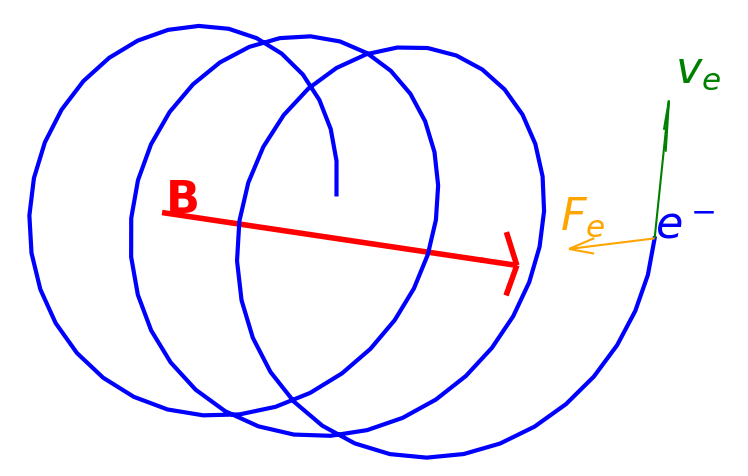
\includegraphics[width=0.6\linewidth]{figs/epath}
    \caption{An electron moving forwards in a solenoidal magnetic field,
        with its velocity $v_e$ and Lorentz force $F_e$. Solenoidal field axis $B$ in red.}
    \label{fig:epath}
\end{figure}

Because the magnets in the cooler are solenoids, the electrons will follow a
spinning path through the cooler according to the Lorentz Force, as seen in
figure \ref{fig:epath}. The higher the transversal momentum of the electrons,
the greater the Lorentz force keeping them inside the specified path.
Great care is taken to ensure that the electron cloud has the desired
beam velocity. Any beam particles that deviates from the desired
velocity, both axially and transversally, will transfer a higher amount
of momentum to the electrons. Beam particles that already have the desired
velocity and low transversal momentum, will see the electrons as stationary,
and thus go through the cooler relatively unchanged. \cite{d_functional_2023-fs}
The functional operation
of the electron cooler is very dependent on the field quality in the
main drift solenoid. Any non solenoidal field components will throw
the electrons off their intended path, thus necessitating high quality
magnetic measurements of the cooler.
\subsection{The new AD cooler}
The path of the solenoid windings, it's placement and manufacturing
irregularities all contribute to non solenoidal field components.
Additionally, the fringe fields of the surrounding magnets in the
toroidal sections also add unwanted field harmonics. Because of this,
a way of compensating for these components are needed.

\newpage
\begin{wrapfigure}{l}{0.4\textwidth}
    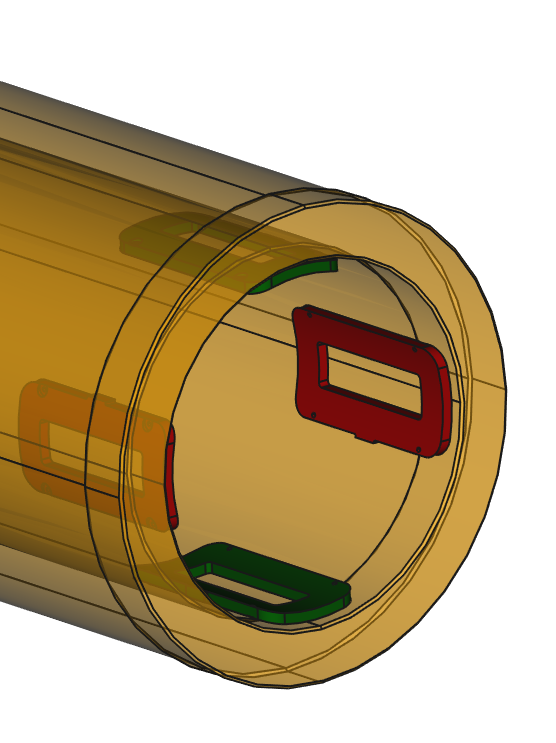
\includegraphics[width=0.9\linewidth]{figs/dipolecorrectors}
    \caption{Dipole correctors (red and green) at the end of a
        solenoid.}
    \label{fig:dipolecorrectors}
\end{wrapfigure}

The new AD cooler is still in its design phase. In the first pass,
the main drift solenoid was made up of several smaller "pancake"
solenoids, as seen in figure \ref{fig:ecooler}. These pancakes could
be individually tilted along their yaw and pitch axes, as well as moved.
The alignment of this pancake array would be done by measuring each
pancake at different tilt/swing angles, to get a field transfer function
with respect to the pancake orientation. These transfer functions would
then be linearly combined, to get the most optimal geometric configuration
for each coil.

The most recent design, at the time of writing instead makes use of
one long drift solenoid, along with several dipole correctors along the
length of the magnet, as illustrated in figure \ref{fig:dipolecorrectors}.

\section{The Measurement System}
The measurement system consists of a PCB fluxmeter with 21 coils printed on it.
This PCB is then moved laterally through the magnet aperture.
The coils then intercept the magnetic flux inside the aperture,
which can be read as a voltage. By keeping track of the fluxmeter's
geometric position, a field map with respect to the aperture length
can be acquired for each coil.

\begin{figure}[!h]
    \centering
    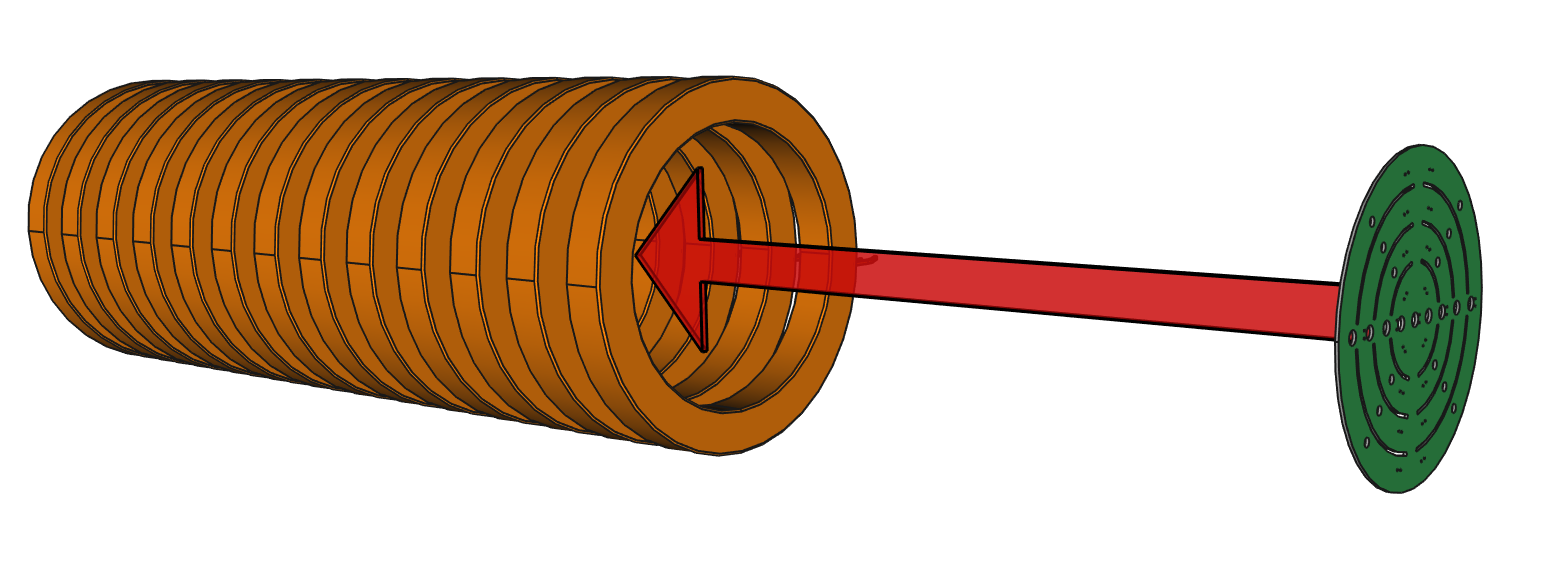
\includegraphics[width=0.6\textwidth]{figs/pcbpath}
    \caption{The fluxmeter entering the magnet aperture.}
    \label{fig:pcbpath}
\end{figure}

\section{Project Purpose and Goal}
The stringent requirements on the field of the AD cooler means the
magnetic measurements must be of high quality. Given that this is
a relatively new measurement methodology, meterological characterization
must be done to evaluate the system. The first design of the AD cooler
would have required measurements of field with respect to the tilt/swing
angle of each individual pancake solenoid. Even though this design was
later discarded, the question of mapping the field measurements to
the misalignment of the solenoid was still deemed to be of interest.
One goal is thus to find out if the pitch and yaw of a solenoid magnet
can be estimated using the magnetic measurements of the fluxmeter.
With such an approach, a solenoid could then be aligned correctly
to the beam aperture with iterative measurements and calibrations.
In the same vein, the minimum detectable angle is of course of interest,
as well as the sensitivity and accuracy of the field measurements.

The initial proposal for measuring the relative pitch/yaw was to
use two coils on opposite sides of the axis, as in figure \ref{fig:coil-dz}.

\begin{figure}[!h]
    \centering
    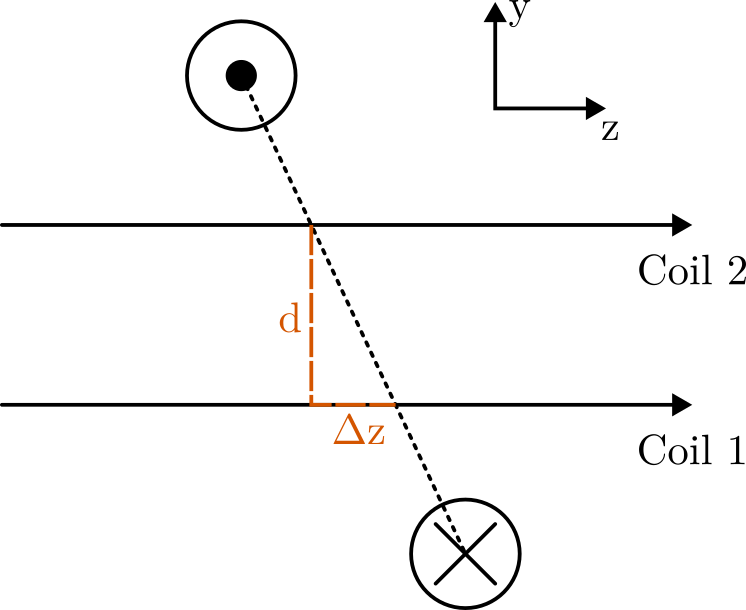
\includegraphics[width=0.6\textwidth]{figs/coil-dz}
    \caption{Two coils measuring the $\vb{B}$ field at different offsets
        from the axis.}
    \label{fig:coil-dz}
\end{figure}

The field in a solenoid is strongest in the middle. As coil 1
and 2 moves through the aperture, they will hit the peak field at different
times. Through some simple trigonometry, the relative tilt between the
solenoid and fluxmeter axis can then be estimated from the distance between
the peaks $\Delta z$ and the distance between the coils $d$.
\begin{equation}
    \theta = \arctan \left( \frac{d}{\Delta z} \right)
\end{equation}

Where $\theta$ is the relative tilt angle.
This model was not tested however, and thus needed to be verified.


Some work has already been done on the system, for instance on measuring
the longitudinal and transversal field components, as well as estimating
the field axis. \cite{petrone_induction-coil_2022}
\chapter{Background}

\section{Electromagnetic Fields}
The electromagnetic fields are a collection of closely linked fields.
These fields govern the electric and magnetic interactions of charged
particles and domains. These fields can be seen in table \ref{tab:fields}

\begin{center}
    \begin{tabular}{c c c}
        \label{tab:fields}
        Field    & SI unit         & Description              \\
        \hline
        $\vb{H}$ & $1\, Am^{-1} $  & Magnetic Field           \\
        $\vb{E}$ & $1\, Vm^{-1} $  & Electric Field           \\
        $\vb{B}$ & $1\, Vsm^{-2} $ & Magnetic Flux Density    \\
        $\vb{D}$ & $1\, Asm^{-2} $ & Electric Flux Density    \\
        $\vb{J}$ & $1\, Am^{-2} $  & Electric Current Density \\
        $\rho$   & $1\, Asm^{-3} $ & Electric Charge Density
    \end{tabular}
\end{center}
These fields are described by Maxwells Equations.
In differential form for the stationary case, these are as follows:

\begin{align}
    \nabla \times \vb{H} & = \vb{J} + \frac{\partial}{\partial t}\vb{D}
    \label{eq:maxwell1}                                                    \\
    \nabla \times \vb{E} & = -\frac{\partial}{\partial t}\vb{B}
    \label{eq:maxwell2}                                                    \\
    \nabla \vb{B}        & = \vb{0}
    \label{eq:maxwell3}                                                    \\
    \nabla \vb{D}        & = \rho
    \label{:eqmaxwell4}
\end{align}
Since we're dealing with measurement of magnetic fields in this thesis,
equations \ref{eq:maxwell1} and \ref{eq:maxwell3} will naturally be of
the most interest. In simple cases, the $\vb{H}$ and $\vb{B}$ field
obey the easy relation 
\begin{equation}
    \vb{B} = \mu \vb{H}
    \label{eq:BHmap}
\end{equation}
where $\mu$ is the \emph{magnetic permeability} in the domain of interest.
Formally, simple cases are where the fields are located in a medium that is
linear, homogenous across its domain, invariant depending on direction, and
stationary. Since the magnetic measurements are made inside the empty aperture
of the magnet, the domain is only made up of air. Thus, equation \ref{eq:BHmap}
holds, and the magnetic permeability is the one of free space, that is
$\mu = \mu_0 = 4\pi \times 10^{-7} Hm^{-1}$. \cite[Ch.4]{russenschuck2011field}


\subsection{The magnetic field and induction}
\subsection{Series decompositions of the magnetic field}
\subsubsection{Cylindrical Coordinates}
\subsubsection{Bessel Functions}
\subsubsection{Bessel-Fourier-Fourier Series}

\section{Signal Processing}
\subsection{Filters}
\subsection{Least Squares Fitting}
\chapter{The Translating Coil Fluxmeter}
The fluxmeter consists of several components. A PCB with
printed flux pickup coils, fast digital integrators, a rotary
encoder and a laser tracker system for geometric positioning measurements.

\begin{figure}[!h]
    \centering
    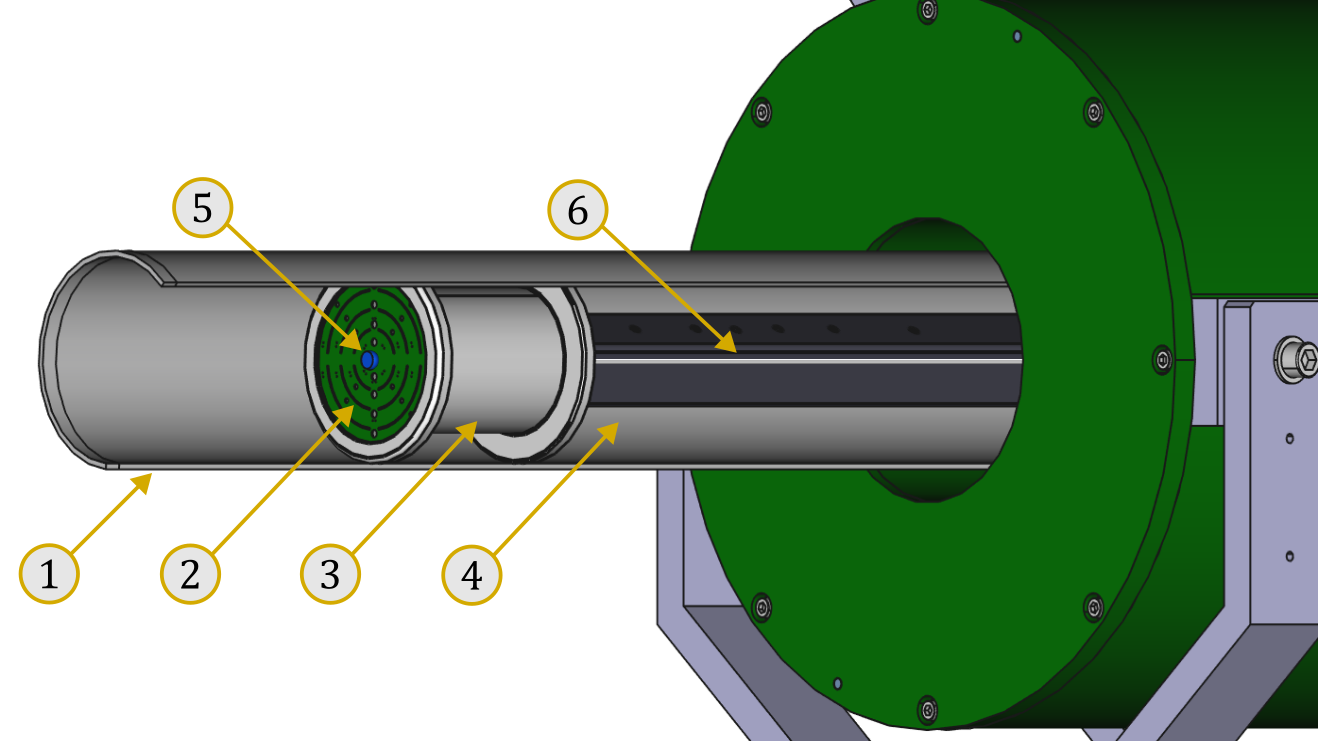
\includegraphics[width=0.7\textwidth]{figs/elena}
    \caption{The fluxmeter assembly going through a solenoid magnet. \\
        1. Guiding Tube, 2. Fluxmeter PCB, 3. PCB Sledge, 4. Supporting arm,
        5. Laser Reflector, 6. Encoder Wire.}
    \label{fig:elena}
\end{figure}

To move the PCB through the magnet aperture, a support assembly was made as
seen in figure \ref{fig:elena}. The coil cables are run through the supporting
arm, which is also used to push and pull the fluxmeter through the tube. A
wire is connected to the PCB sledge on one end, and spooled up around
a rotating encoder on the other end. In the middle of the PCB, a
reflector is mounted for the laser tracker.

\section{PCB printed coils}
The coil PCB has 21 different coils.
These coils are in the shapes of disks or annulus segments.
A render of the pcb can be seen in figure
\ref{fig:pcb}. The disks are denoted $D_l$ and the
annulus segments by $Q_{q, l}$ where $l$ is the radial layer and
$q$ is the quadrant, as seen in figure \ref{fig:nomenclature}.

\begin{figure}[!h]
    \centering
    \begin{subfigure}[b]{0.5\linewidth}
        \centering
        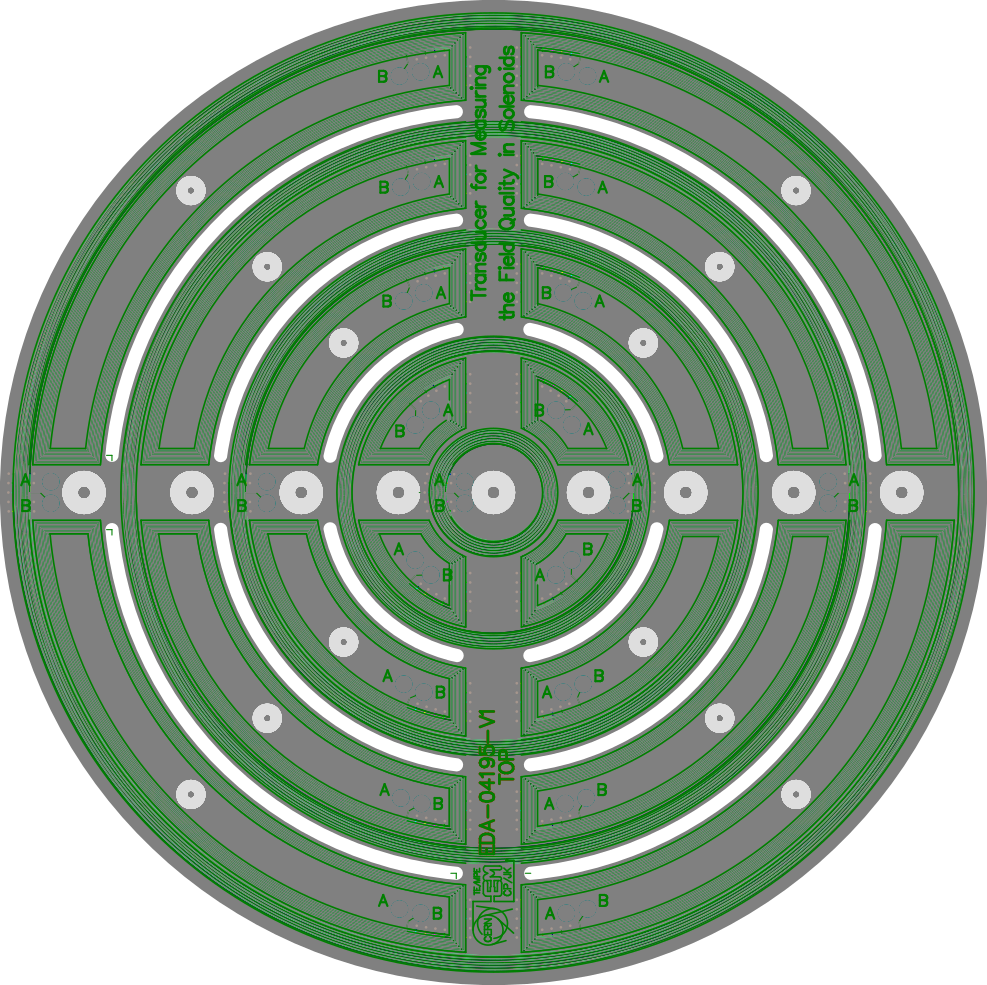
\includegraphics[width=0.8\linewidth]{figs/pcb}
        \caption{The fluxmeter PCB.}
        \label{fig:pcb}
    \end{subfigure}
    \hfill
    \begin{subfigure}[b]{0.4\linewidth}
        \centering
        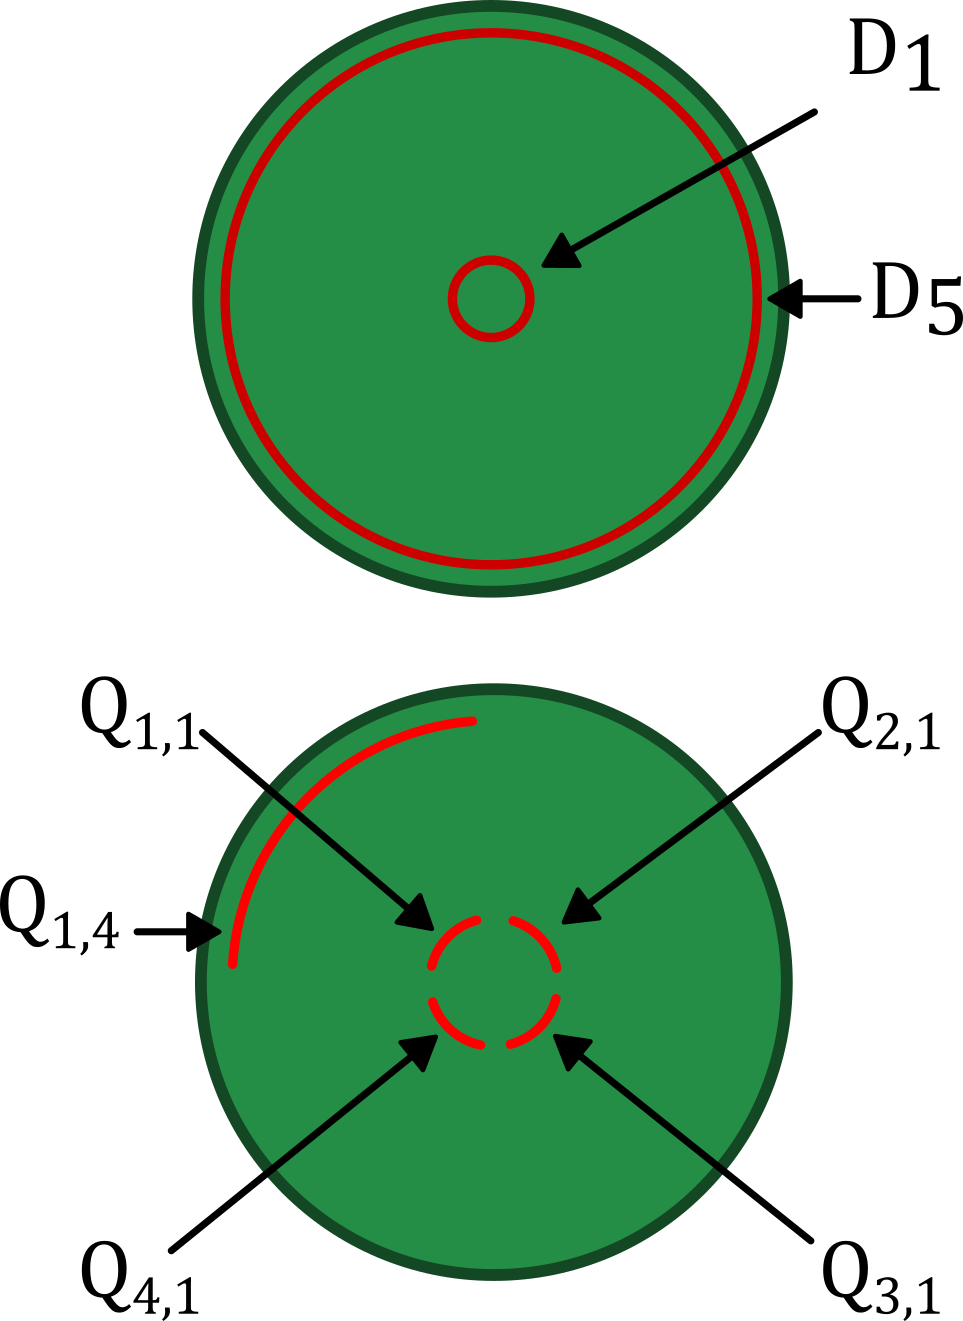
\includegraphics[width=0.8\linewidth]{figs/nomenclature.png}
        \caption{Nomenclature of the PCB coils.}
        \label{fig:nomenclature}
    \end{subfigure}
    \caption{}
\end{figure}

During measurements, the magnet is magnetized with a constant current.
As the coils move through the magnet, a voltage is induced according
to Faradays Law, equation \ref{eq:faraday}. Although the field is
static, since the fluxmeter is moving it will still see a delta
flux with respect to time.

\section{The Measurement Assembly}
A picture of the magnet with the guiding tube and tube clamps can be seen in
figure \ref{fig:magnetassembly}. In figure \ref{fig:leica}, the laser tracker
can be seen, locked onto the target on the fluxmeter pcb.

\begin{figure}[!h]
    \centering
    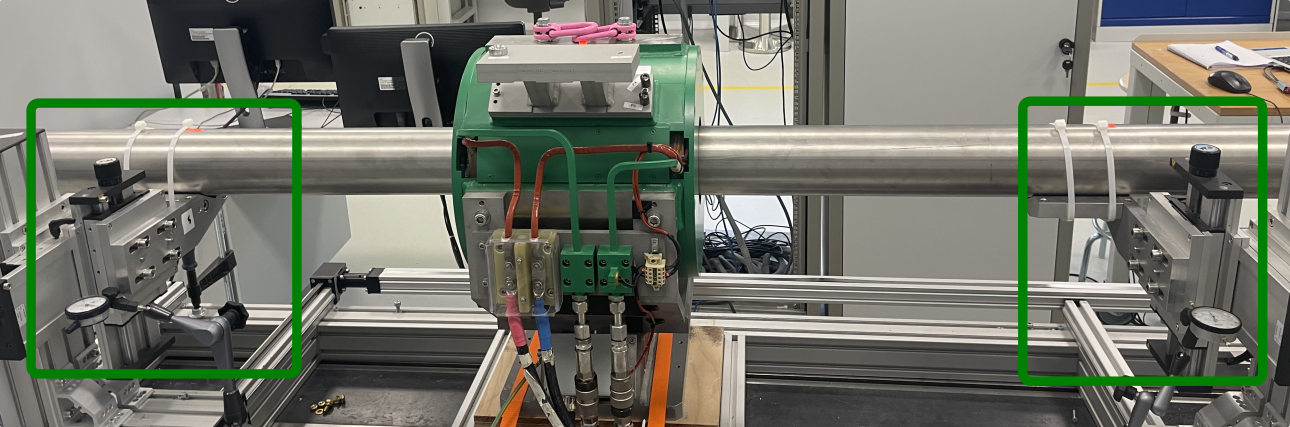
\includegraphics[width=0.7\textwidth]{figs/magnet-assembly}
    \caption{Guiding tube in the magnet. Tube clambs marked in green rectangles.}
    \label{fig:magnetassembly}
\end{figure}

\begin{figure}[!h]
    \centering
    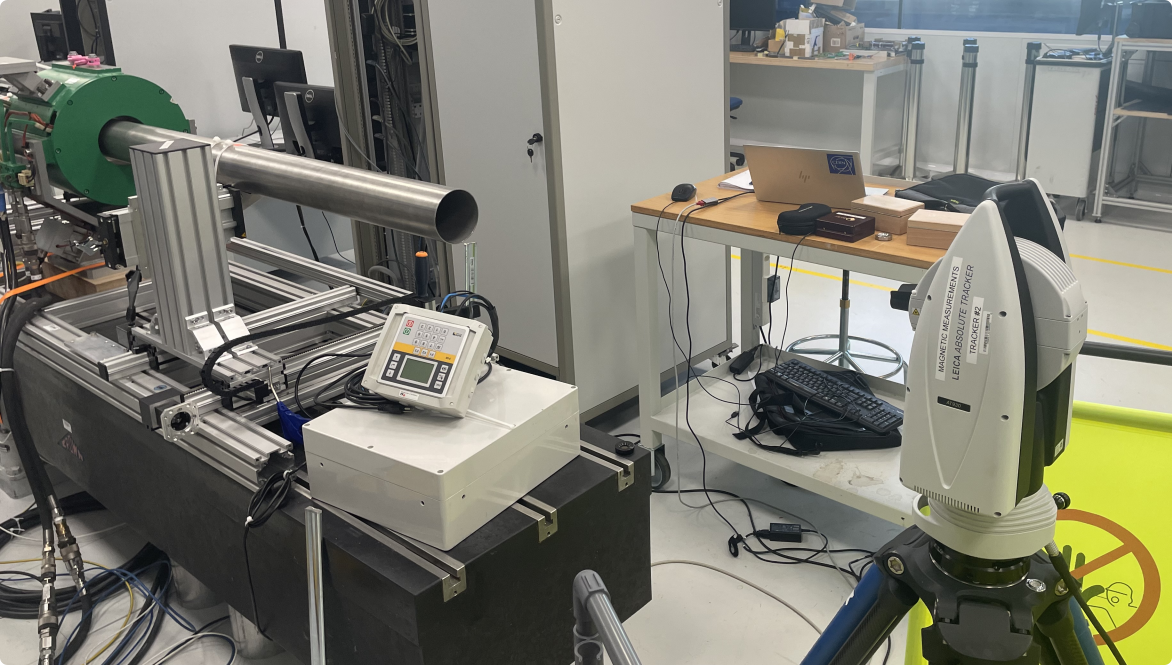
\includegraphics[width=0.7\textwidth]{figs/leica}
    \caption{Laser tracker, looking into the guiding tube.}
    \label{fig:leica}
\end{figure}

\section{Geometric Measurements}
The laser tracker works by shooting a laser at a reflector, and then
measuring the time of flight. The accuracy depends on the reflector
type and measurement time, but an upper limit of
0.2 mm is a reasonable estimate according to the
specifications of both the reflectors and laser tracker
used. \cite{noauthor_leica_2015}.

Firstly, scans were done of a network of reflectors around the
room. These points were then used as a baseline to locate the
laser tracker at the start of each measurement campaign, or when
the laser tracker needed to be moved. A cluster of points were
taken of the magnet itself. These points
were then fitted to a cylinder. Using a 3D model of the
solenoid, a coordinate system could be constructed
with its origin at the geometric center of the magnet.
The $z$ axis was chosen as the solenoidal axis, pointing
in the field direction. $y$ was chosen as the axis
pointing up, opposite to gravity, leaving $x$ as 
the axis parallel to the ground.

Furthermore, two planes were constructed at the positions
of the clamps holding the fluxmeter guiding tube. The
positions of these clamps could accurately be moved in
both lateral dimensions using precision dials. In effect,
the tube has two anchor points that can be moved along
the aforementioned planes, so that it can be aligned (or misaligned)
as desired.

\begin{figure}[!h]
    \centering
    \includegraphics[width=0.7\textwidth]{figs/3Dscan}
    \caption{3D scans of the measurement assembly.
        1: Laser Tracker, 2: 3D scan of the solenoid,
        3: Network Point, 4: Tube clamp positioning planes.
        3D scans fitted using Spatial Analyzer \cite{hexagon_spatial_nodate}.}
    \label{fig:3dscan}
\end{figure}

\section{Positional Encoder}
The positional encoder is a rotating encoder connected to a wire spool.
As the fluxmeter moves through the the magnet, it pulls on the wire,
spinning the rotating encoder. The encoder is of a 16 bit type, meaning
it sends out a pulse $2^{16} = 65536$ times per turn. These pulses were
decimated by a factor of 32, giving 2048 pulses per turn. By triggering
the laser tracker with these pulses, it was found that one turn corresponds
to a fluxmeter translation of $23.0095$ cm along the axis. The distance
per pulse were measured to be $0.11$ mm, with a standard deviation of
$6.69 \, \mu \text{m}$.

\begin{figure}[h]
    \centering
    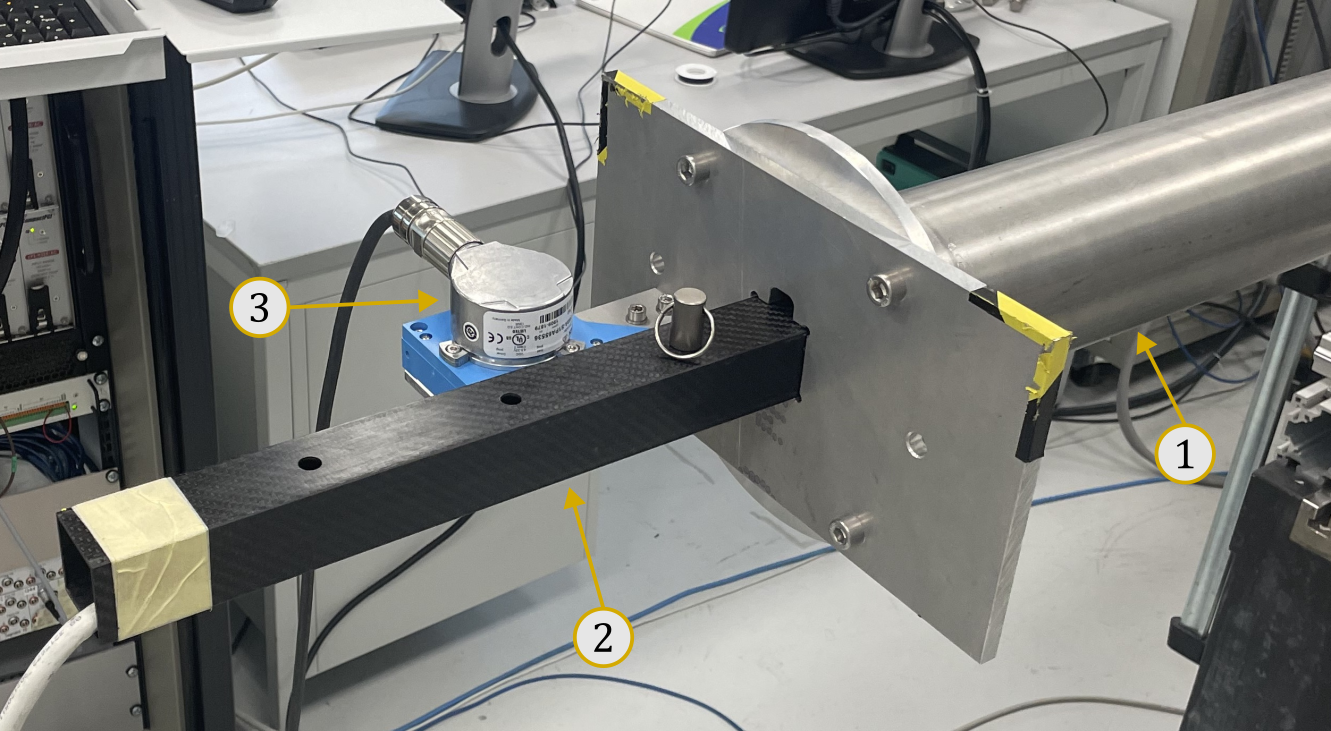
\includegraphics[width=0.7\textwidth]{figs/encoder}
    \caption{One end of the fluxmeter guiding tube (1), with guiding arm (2)
        and positional encoder (3).}
    \label{fig:encoderpic}
\end{figure}

\section{Fast Digital Integrators}
The fast digital integrators (FDI:s) are used to align flux measurements
with their geometric positions. They continuously sample the voltages
from the fluxmeter coils at $500$ kHz. For every trigger from the encoder,
the FDI:s outputs the integrated voltage with respect to time, with the
integration limits being the last two triggers. This
corresponds to the change in flux between two trigger times $t_i$. Since these
triggers are fired at specific points along the fluxmeter axis, the
delta fluxes can easily be mapped from time to geometric position, as in
equation \ref{eq:deltaPhi}.

\begin{equation}
    \Delta \Phi_i =
    \int \limits_{t_{i-1}}^{t_i} \frac{d}{dt}\Phi dt
    = \Phi_{z_{i-1}} - \Phi_{z_{i}} = \Delta \Phi[z_i]
    \label{eq:deltaPhi}
\end{equation}

The flux through a coil for each $z$ position is then easily obtained
by taking the cumulative sum of the delta fluxes, as in equation
\ref{eq:Phiz}.

\begin{equation}
    \Phi[z_i] = \sum \limits_{k=0}^i \Delta \Phi[z_i]
    \label{eq:Phiz}
\end{equation}

The advantage of this approach is that the measurements are invariant
to the speed at which the fluxmeter moves through the magnet, within limits.
The lower limit on the translating speed is such that the induced
voltage in the coils is higher than the noise floor.
The upper limit is decided by the sampling frequency of the FDI:s.
As long as a sufficient number of voltage samples are gathered between
each encoder trigger, the measurements are repeatable to a high accuracy.

Furthermore, the integration operation of the FDI:s act as a
low pass filter, removing high frequency noise in the voltage
signals.

As seen in figure \ref{fig:measurement-assembly}, the encoder triggers
both the FDI:s and the laser tracker, giving accurate positions coupled
to the delta fluxes. This way, the geometric repeatability of the 
measurements were substantially increased, since the laser tracker 
had fixed coordinate frame in relation to the network points.

\tikzset{sensor/.style={rectangle, rounded corners, minimum width=3cm, minimum height=1cm,text centered, draw=black, fill=green!30}}
\tikzset{process/.style={rectangle, minimum width=3cm, minimum height=1cm, text centered, draw=black, fill=orange!30}}
\tikzset{output/.style={diamond, minimum width=3cm, minimum height=1cm, text centered, draw=black, fill=white!30}}

\begin{figure}[h]
    \centering
    \begin{tikzpicture}[node distance=3cm]
        \node (coils) [sensor, align=center] {Fluxmeter\\PCB};
        \node (encoder) [sensor, below of=coils] {Encoder};
        \node (triggers) [right of=encoder] {Triggers};

        \node(leica) [process, right of=triggers, align=center]
        {Laser\\Tracker};

        \node(FDI) [process, right of=coils, xshift=3cm]
        {FDI:s};

        \node(output) [output, right of=FDI, yshift=-1.5cm] {Output};
        \coordinate [below of=FDI, yshift=1.5cm] (bFDI);

        \draw [->] (coils) -- node[anchor=south]{Voltages}(FDI);
        \draw [->] (FDI) -| node[anchor=south]{$\Delta$ Fluxes} (output);
        \draw [->] (encoder) -- (triggers);
        \draw [->] (triggers) -- (leica);
        \draw [->] (triggers) |- (bFDI) -- (FDI);
        \draw [->] (leica) -| node[anchor=north]{Positions} (output);
    \end{tikzpicture}
    \caption{Flowchart for the measurement assembly.}
    \label{fig:measurement-assembly}
\end{figure}
\chapter{Measurements}
Several measurement campaigns were done to characterize the system.
A number of measurements were done at different solenoid tilt
angles, to estimate the effect of tilt-swing misalignment on 
the peak shifts of coils. Maps with all 21 coils
were done at a number of angles, as well as repeated measurements
for accuracy estimation. A number of procedures had to be developed
in order to make the measurements repeatable. 

\section{Fluxmeter Accuracy Estimation}
To estimate the accuracy and repeatability of the fluxmeter, 10
measurements were done under similar conditions. Coils D1-D5 as
well as Q44 were used since these have a large spread in total coil area.
The normalized standard deviation was then calculated for each coil.
Figure \ref{fig:coilarea} shows the standard deviation as a function 
of coil area.

\begin{figure}[!h]
    \centering
    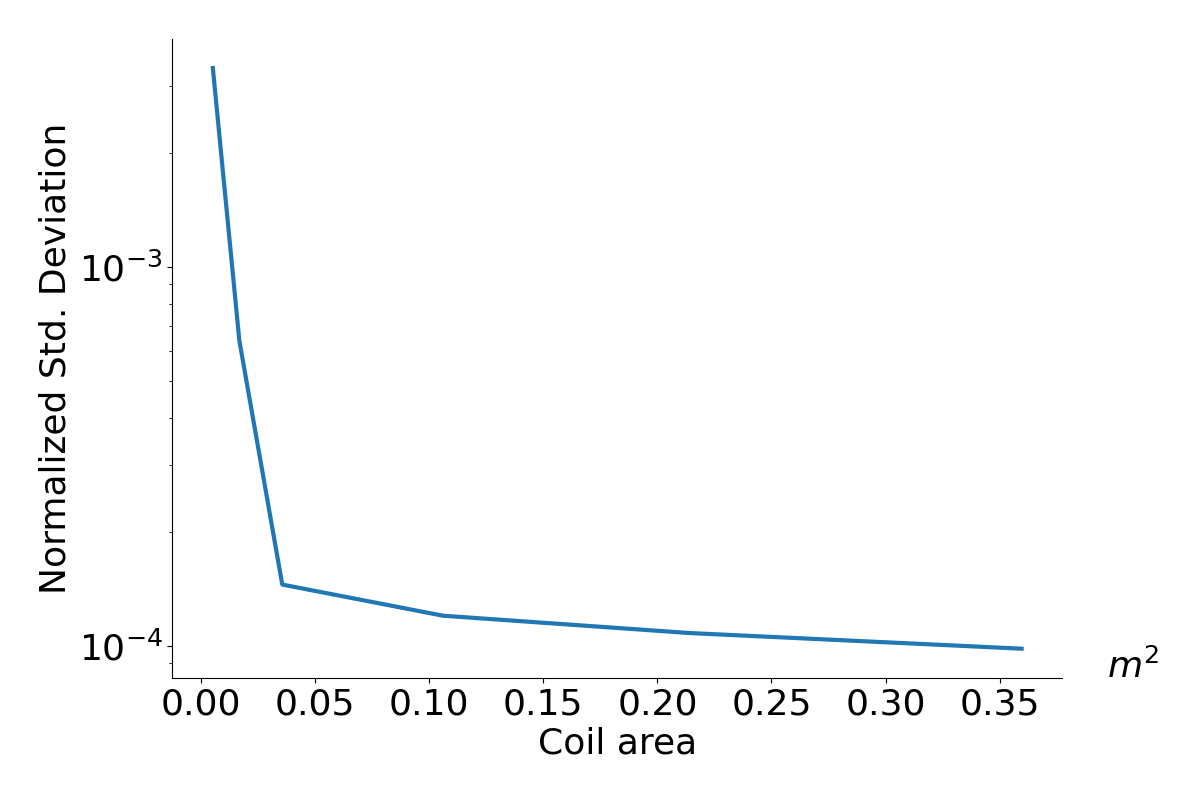
\includegraphics[width=0.8\linewidth]{figs/coilarea-error}
    \caption{Normalized measurement std. deviation as a function of
    coil area.}
    \label{fig:coilarea}
\end{figure}

As can be seen, the standard deviation of the measurements starts
increasing very fast as the coil surface area gets lower than
about $0.02$ $\text{m}^2$. A likely cause is that the signal
is starting to reach the same magnitude as the noise at this
point, which means that this is a reasonable lower bound 
on the coil surface are for a magnet of this strength ($80$ mT). 
For the region where the signal to noise ratio is high, the
standard deviation is reliably in the low promilles.

\section{The Fluxmeter Alignment Procedure}
An alignment procedure was developed for the fluxmeter, so that
measurements could be taken in an aligned, almost ideal case
or with a desired tilt angle around the $y$ axis. This will 
hereafter be referred to as the yaw angle. 

First, the laser tracker is used to sample the fluxmeter positions
as it is translated through the guiding tube. These samples are then fitted to
a line in three dimensional space, as in figure \ref{fig:geomfit}.

\begin{figure}[!h]
    \centering
    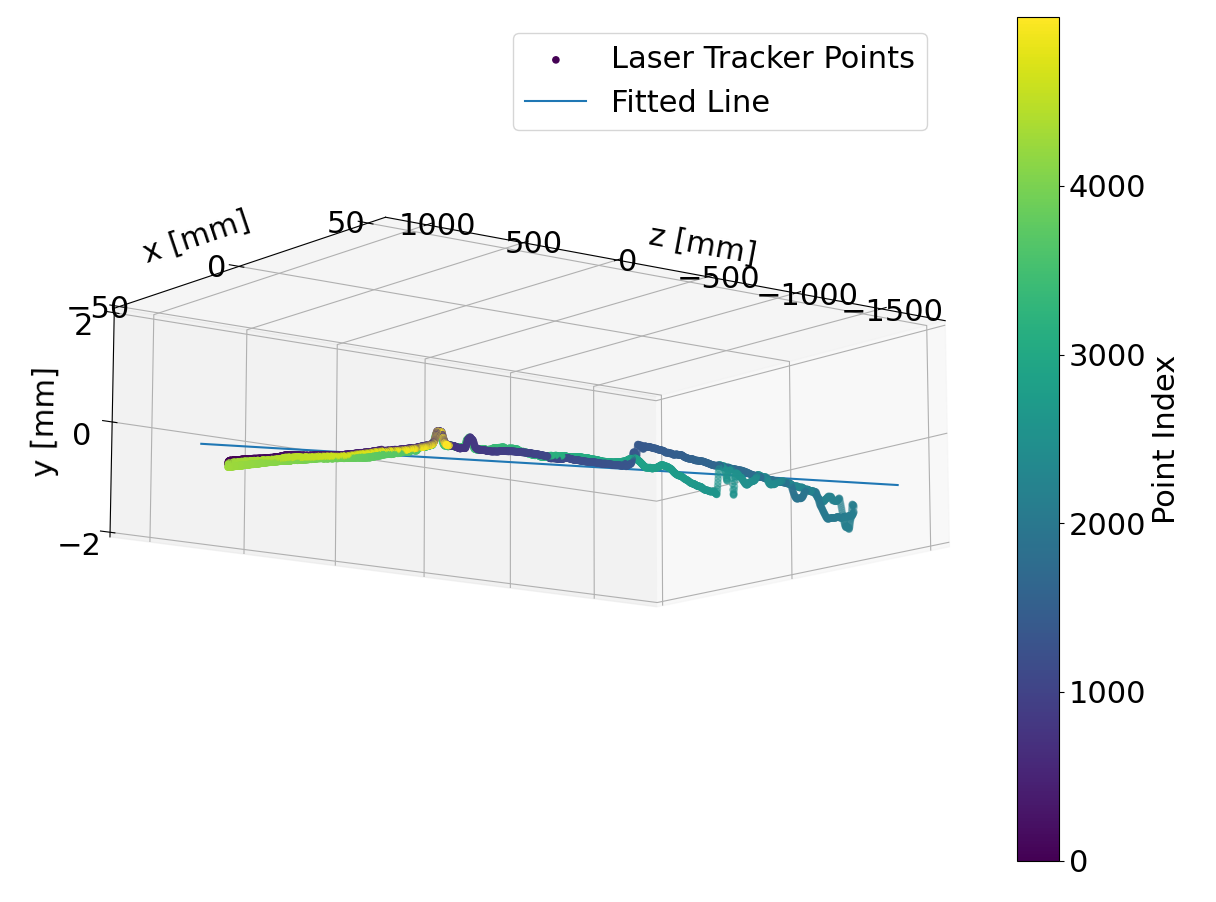
\includegraphics[width=0.8\linewidth]{figs/geomfit}
    \caption{Measured fluxmeter positions along with a line
    fit. The fluxmeter tube is tilted by $30$ mrad around the y axis.}
    \label{fig:geomfit}
\end{figure}

The intersections between the fluxmeter path line and the 
planes $z = z_{Back}$, $z = z_{Front}$ are then found, where
$z_{Back}$ and $z_{Front}$ are the $z$ offsets where the tube clamps
are located. The measured intersections $\tilde{p}_1$ and $\tilde{p}_2$
are illustrated in figure \ref{fig:alignment}.

\begin{figure}[!h]
    \centering
    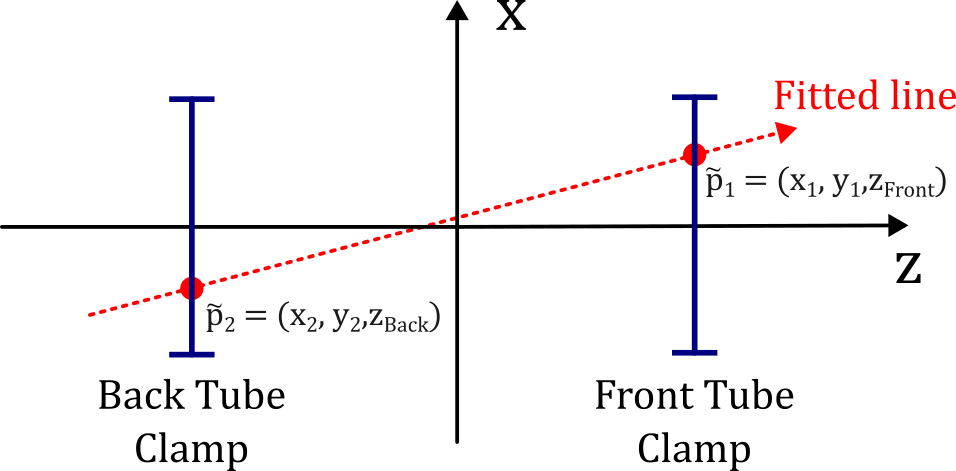
\includegraphics[width=0.8\linewidth]{figs/alignment}
    \caption{The fluxmeter path and its intersection points with
    the tube clamps.}
    \label{fig:alignment}
\end{figure}

The optimal intersect points $p_1, p_2$
are found by simple trigonometry:
\begin{align}
    p_1 = (z_{Front}\tan(\theta), 0, z_{Front}) \\ 
    p_2 = (-z_{Back}\tan(\theta), 0, z_{Back})
\end{align}
where $\theta$ is the desired yaw angle. Calculating the needed
adjustment is then a simple matter of comparing the measured
and optimal intersect points. The front clamp is adjusted by
$\tilde{p}_1 - p_1$ and the back clamp by $\tilde{p}_2 - p_2$.

The fluxmeter path is then measured again with the laser tracker,
and the whole procedure is iterated until the desired yaw angle
is reached, to an accuracy of 
$|\tilde{p}_1 - p_1|, |\tilde{p}_2 - p_2| < 0.2$ mm.
$z_{Front} - z_{Back} = 1521$ mm, making the yaw angle error
less than $0.26$ mrad.

\section{Peak Shift Measurements}
In section \ref{}
\chapter{Simulations}

\section{Solenoid tilt-swing angle and its effect on the $B_z$ field peaks}
\label{sec:simulations}

To further understand why the model presented in equation
\ref{eq:angle_estimation} did not perform as hoped, the relationship
between the $B_z$ field peaks and the yaw angle was investigated in
a simulation campaign. The coil dimensions presented in figure
\ref{fig:sim-mag-dims} were varied in a parametric sweep.
For each sweep, the $z$ value at the field maximum along the lines $l_1$ and $l_2$
was calculated as a function of the yaw angle \emph{Rot}. Each
of the lines were tangential to the $z$ axis with some offset
$y_{off}$ in $y$ as presented in figure \ref{fig:sim-mag-rot}.

\begin{figure}[h!]
    \centering
    \begin{subfigure}[b]{0.4\textwidth}
        \centering
        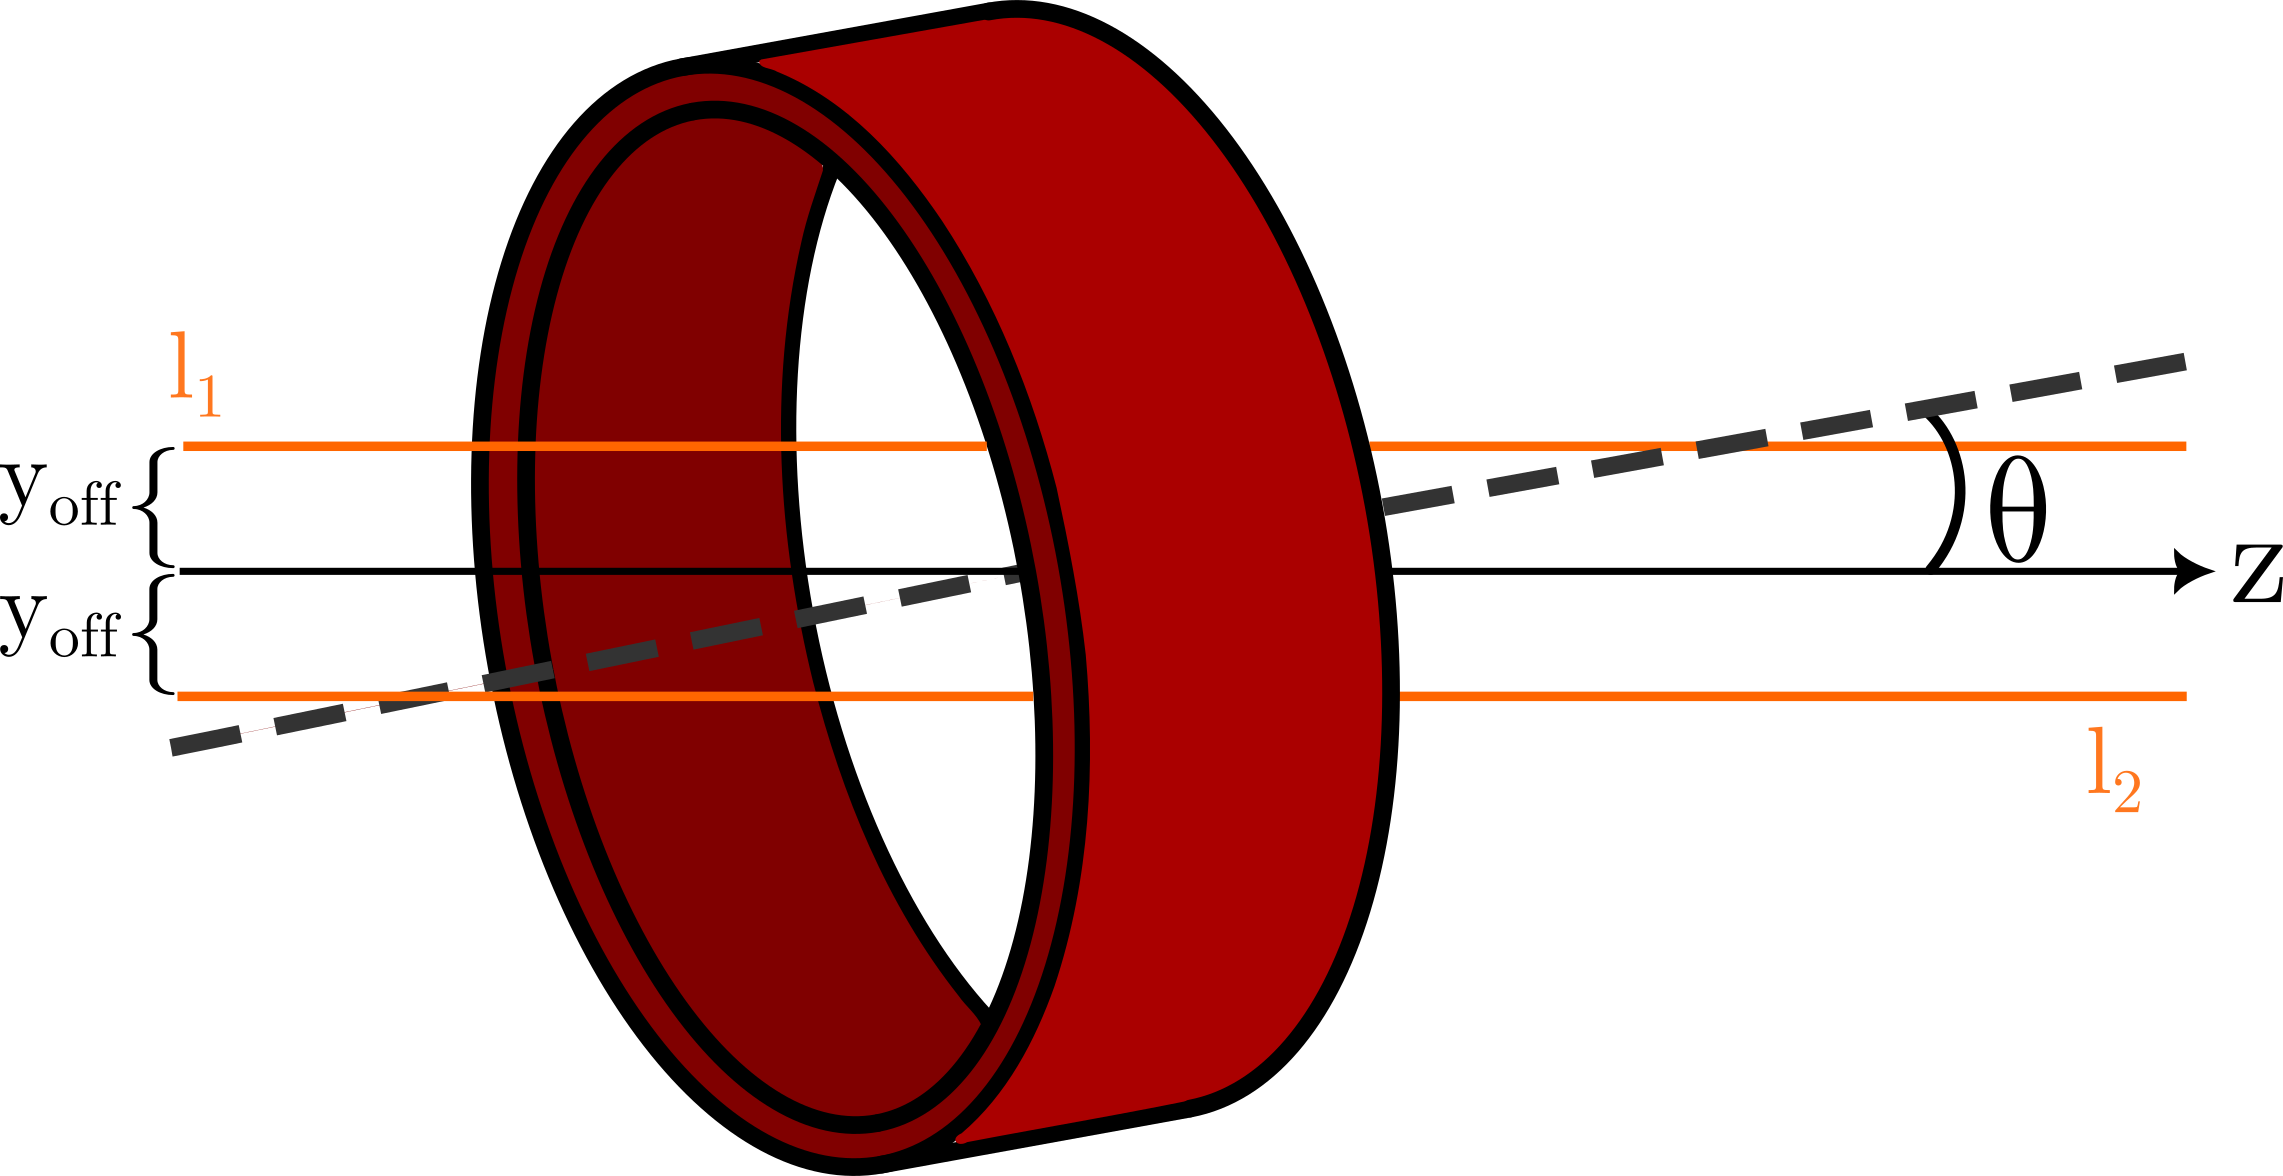
\includegraphics[height=100pt]{figs/sim_mag_rot}
        \caption{Coil placement parameters in simulations.}
        \label{fig:sim-mag-rot}
    \end{subfigure}
    \hfill
    \begin{subfigure}[b]{0.4\textwidth}
        \centering
        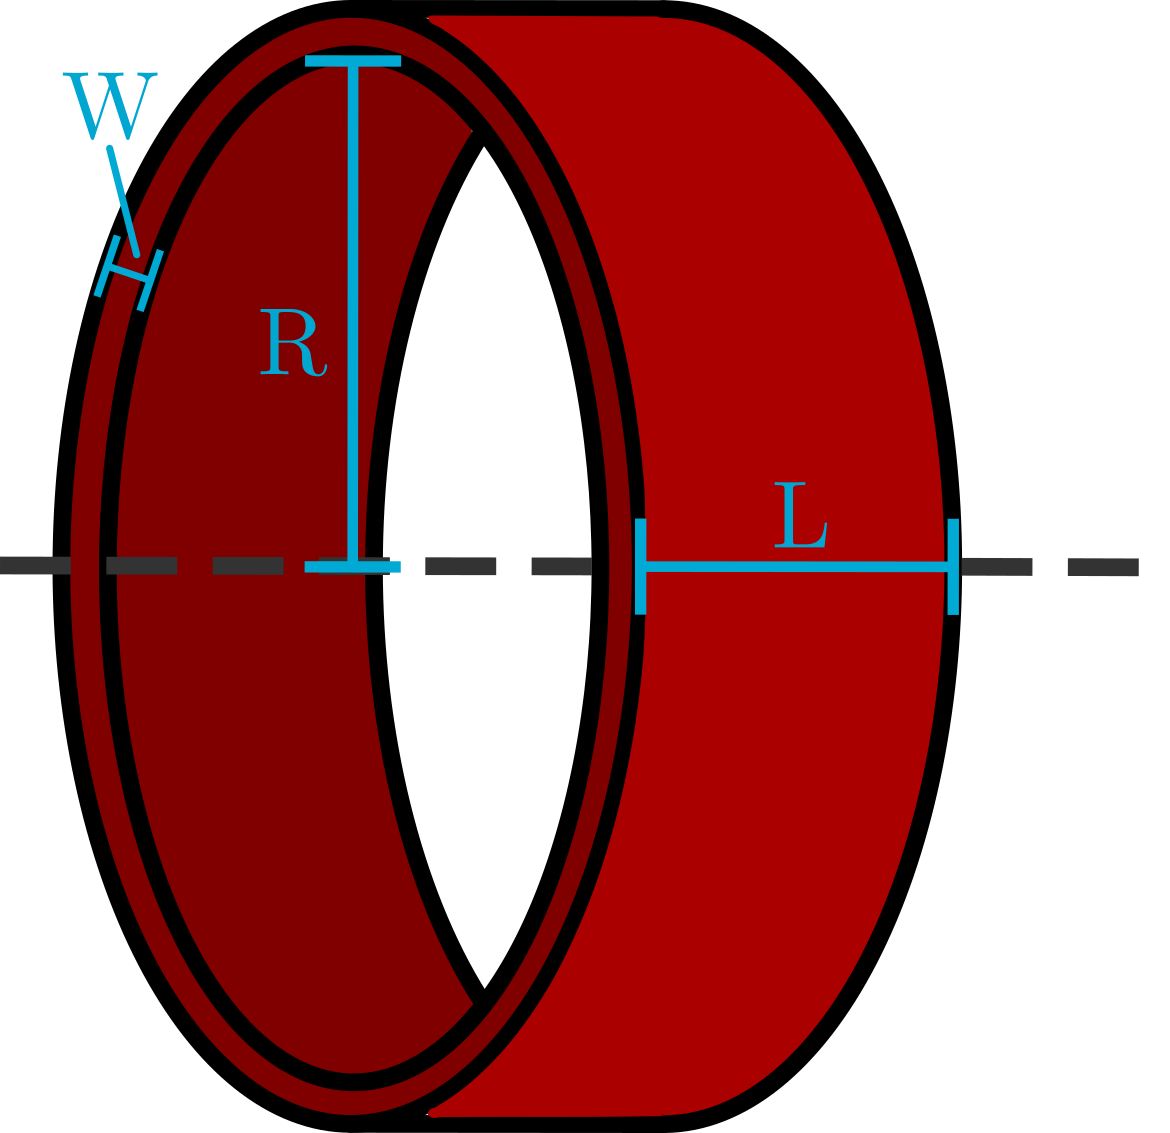
\includegraphics[height=100pt]{figs/sim_mag_dims}
        \caption{Coil dimension parameters in simulations.}
        \label{fig:sim-mag-dims}
    \end{subfigure}
    \caption{}
\end{figure}

The range and unique values for each parameter is presented in table \ref{tab:parameter-vals}.
The parameter values are spaced out evenly across their range. Where necessary, simulation
results have been discarded when the $y$ offsets are too large, such that the lines $l_1$
and $l_2$ go through the numerical singularities inside the magnet.

\begin{table}[h!]
    \begin{center}
        \begin{tabular}{c c c c}
            Parameter              & Shorthand name & Range         & \#Unique Values \\
            \hline
            Magnet Radius          & \emph{R}       & $0.2-0.5$ m   & 21              \\
            Magnet Width/Thickness & \emph{W}       & $0.0-0.4$ m   & 6               \\
            Magnet Length          & \emph{L}       & $0.0-0.5$ m   & 9               \\
            Line $y$ offset        & $y_{off}$      & $0.05-0.2$ m  & 11              \\
            Magnet yaw angle       & $\theta$       & $0.0-0.5$ rad & 31
        \end{tabular}
        \caption{Simulation parameter values}
        \label{tab:parameter-vals}
    \end{center}
\end{table}

The simulations were done numerically, with several thin
current loops spread out at a constant density along the magnet
width $W$ and length $L$. Some randomly chosen results were
verified using FEM simulations with a similar magnet model.

Figure \ref{fig:sim-mag-dimensions} gives an idea of the general impact that the
magnet dimensions have on the peak shifts. For each plot, the other magnet dimensions
are constant. A key takeaway is that most magnet dimensions do not affect
the peak shift that much at the chosen parameter values, especially at
lower yaw angles. The offset from the axis however has a great effect.


\begin{figure}
    \centering
    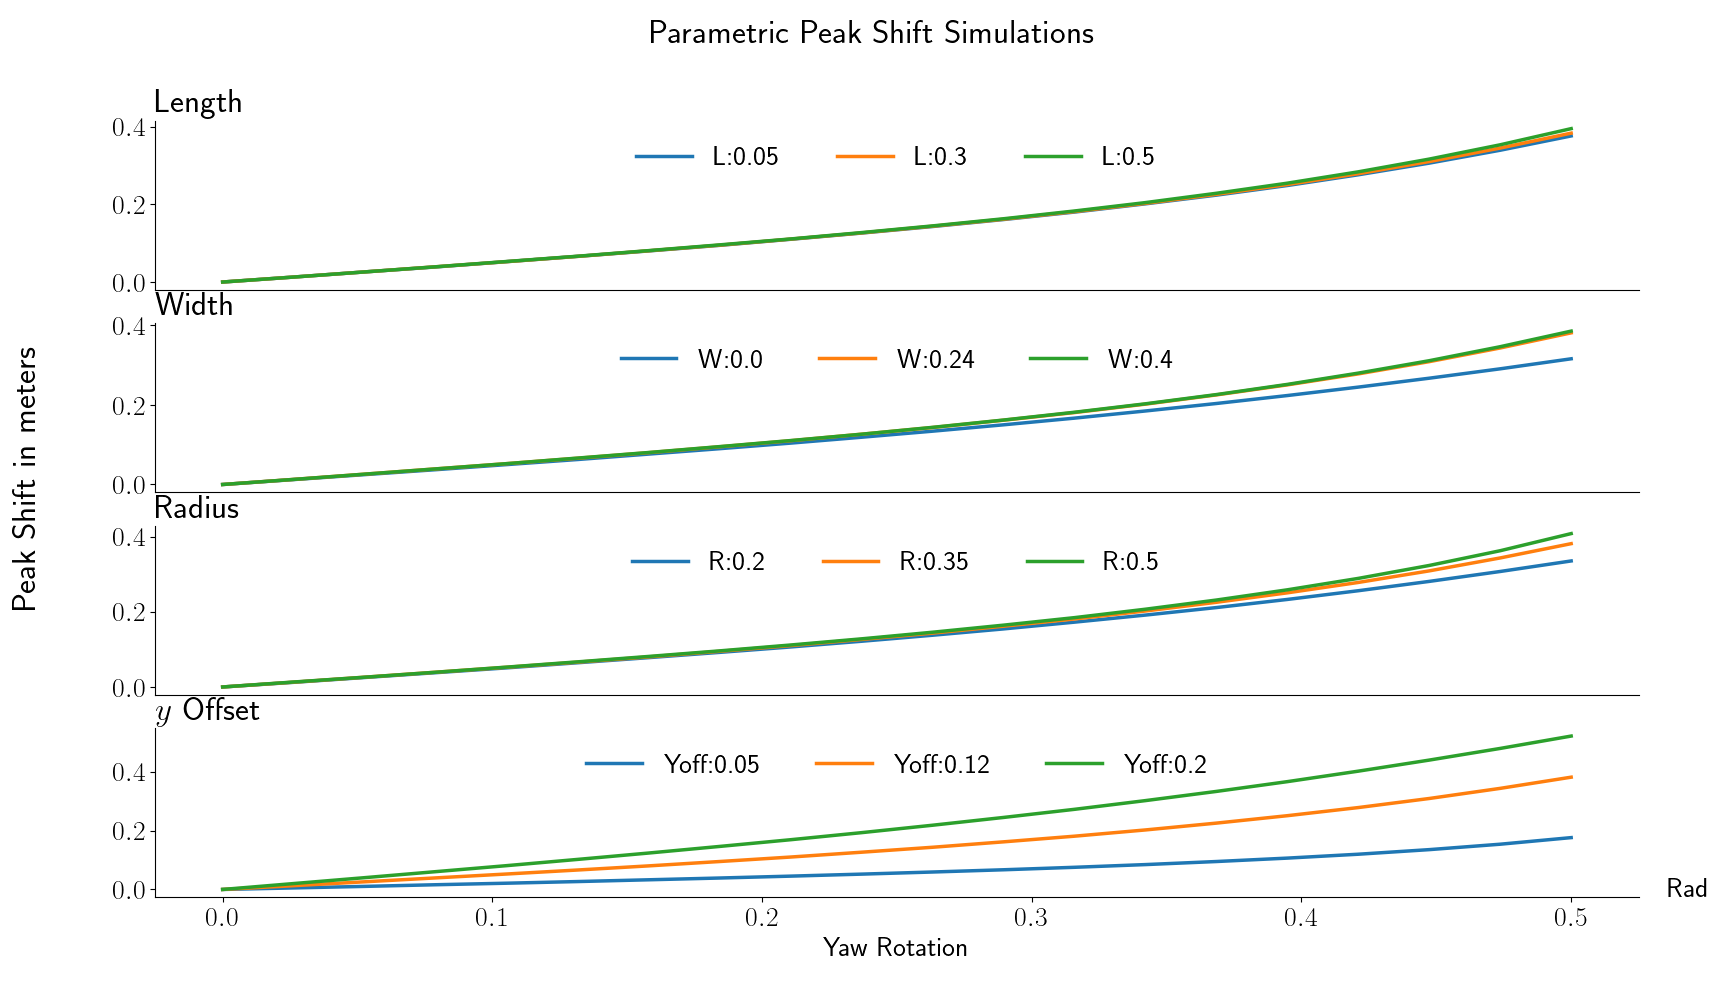
\includegraphics[width=\linewidth]{figs/sim_params_plot}
    \caption{Peak shifts and how they vary with yaw angle and magnet dimensions.}
    \label{fig:sim-mag-dimensions}
\end{figure}

The effect of the $y$ offset can be clearly seen in figure
\ref{fig:sim-mag-fieldmap-argmax}. Unfortunately, it does not seem
that the effect is easily modeled. For a simple current loop, the peak
shifts seem to follow a tangent like function in $y$.
For more realistic solenoid models with a more homogenous
field inside, the the argmax follows a more affine curve,
but still does not follow the geometric solenoid centre.
Clearly, the simple model
presented in equation \ref{eq:angle_estimation} will overestimate
the angle since the $B_z$ peaks are not distributed along the geometric
solenoid centre, but rather further out. The $\Delta z$ argument in
equation \ref{eq:angle_estimation} will thus be larger than the model
expects, regardless of solenoid configuration.


\begin{figure}[h!]
    \centering
    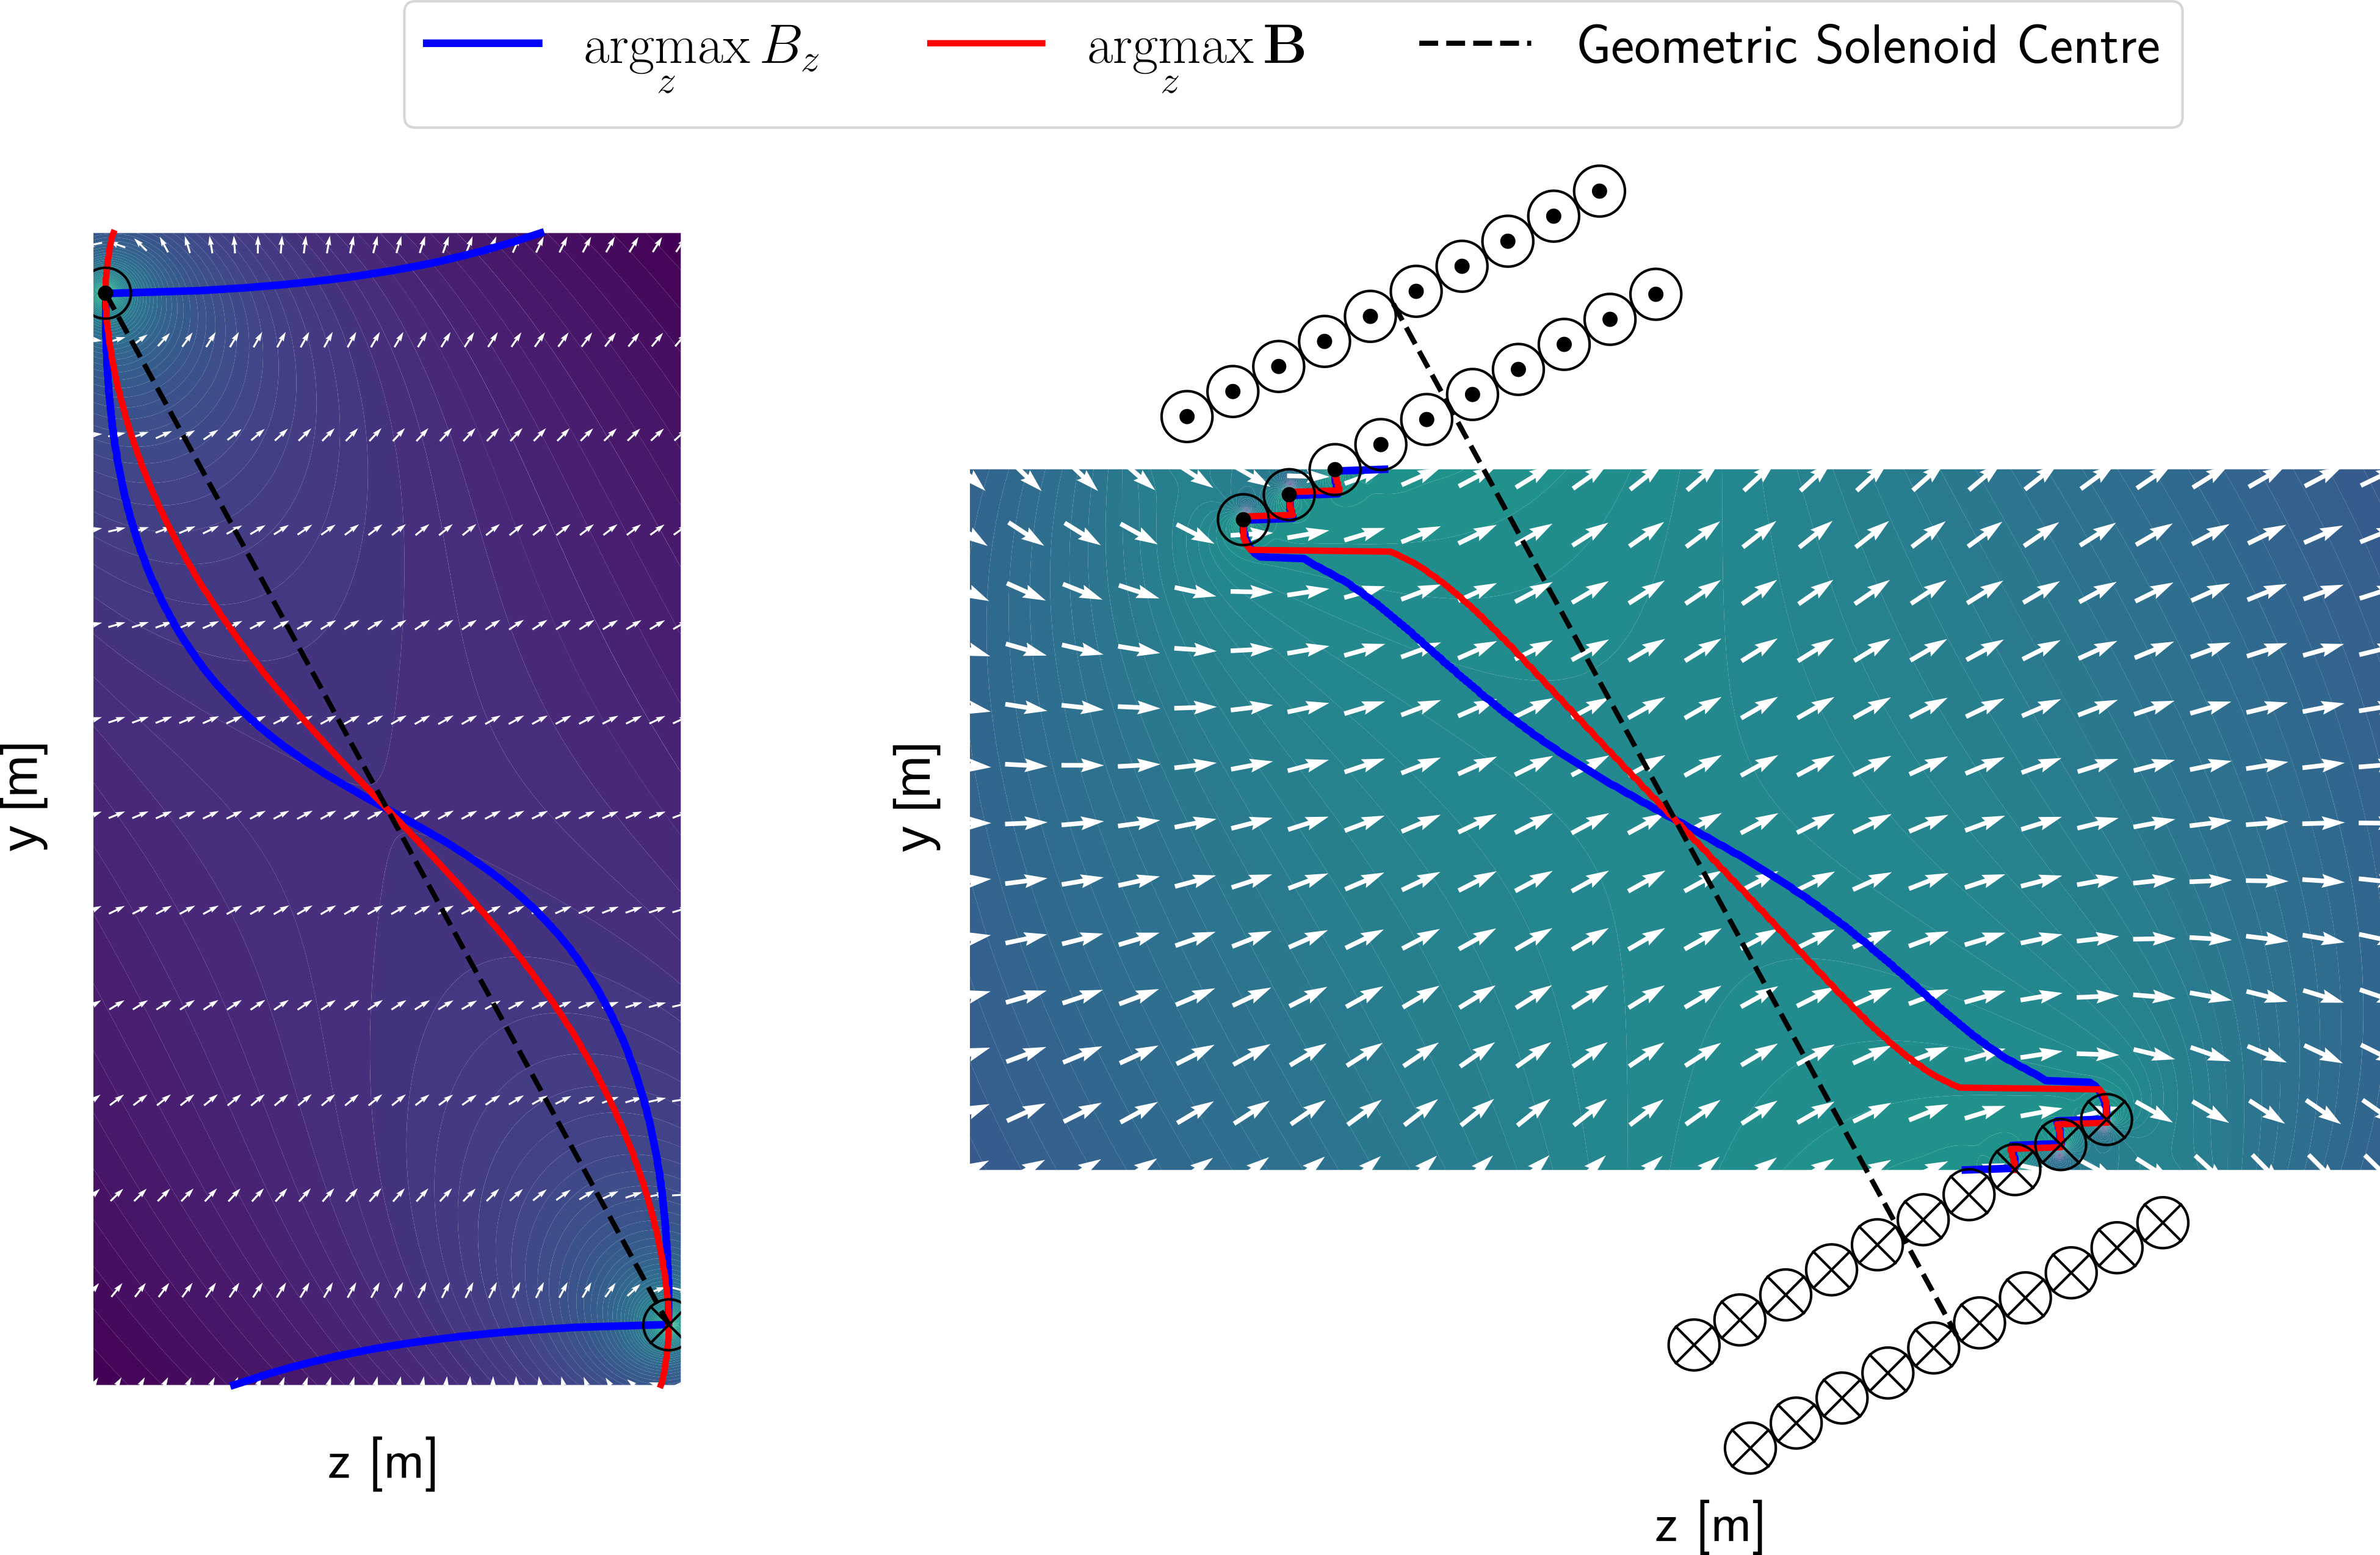
\includegraphics[width=\linewidth]{figs/sim-fieldmap}
    \caption{$\vb{B}$ and $B_z$ argmax over $y$, for a simple current
        loop and coil made up of 600 turns.}
    \label{fig:sim-mag-fieldmap-argmax}
\end{figure}

\section{The transversal integral field and dipoles}
\label{sec:dipole-simulations}
In section \ref{sec:theory-dipoles} it was shown that the integral
$B$ field and subsequently the $z$ dipole in field
series expansions was


\begin{equation}
    \int \limits_{t_0}^{t_1} \vb{B}(\vb{l}(t))dt = C_{0,0}L \approx \mu_0 NI
    \label{eq:Bzlineint}
\end{equation}

for a line integral going through a solenoid, regardless of the yaw
angle $\theta$. $\vb{l}$ is a curve whose image
is a line with length L and whose ends are far from the magnet, where
the magnetic field strength is negligible.

Now, let $\vb{l}$ be parallel with the $z$ axis, and instead take the
transversal integral fields, as in equations \ref{eq:Bx-Integral} and
\ref{eq:By-Integral}.

\begin{align}
    I_{\vb{l}}(B_x) & := \int \limits_{\vb{l}} B_x d\vb{l}
    \label{eq:Bx-Integral}                                 \\
    I_{\vb{l}}(B_y) & := \int \limits_{\vb{l}} B_y d\vb{l}
    \label{eq:By-Integral}
\end{align}

This could be
likened to measuring the $x$ and $y$ field by translating a hall sensor
through the solenoid, and then taking the integral of the measurements.
It was discovered in the work on this thesis, that the aforementioned
integral fields seems to be connected to the yaw/pitch angle of the
solenoid.

This relationship can not easily
be found algebraically, and was instead investigated using the same
simulation setup previously described in this chapter. The numerical integral of
both $B_z$ and $B_y$ were taken along $\vb{l}$ over different yaw angles $\theta$.
Like before, the solenoids
radius, length and width were varied, as well as the $x$ and $y$ offset.
The $x, y$ offsets were small enough
for $l$ to pass through the solenoid aperture.

Regardless of all of the variations between simulation passes, the results were
consistent down to a millionth of a radian.
Furthermore, the value of the $By$ integral along $\vb{l}$
was invariant to the $x,y$ location of $\vb{l_1}$ inside the solenoid.
The simulations suggest that when a solenoid is tilted with an angle $\theta$
around the x axis, the integral of $B_y$ along $\vb{l}$ becomes

\begin{equation}
    \int\limits_{\vb{l}}B_y d\vb{l} =
    \tan\left( \frac{\theta}{2} \right)  \int\limits_{\vb{l}}\vb{B} d\vb{l}
    \approx \mu_0\tan\left( \frac{\theta}{2} \right) NI
    \label{eq:tanhalf}
\end{equation}
or alternatively
\begin{equation}
    \frac{I_{\vb{l}}(B_y)}{\mu_0NI} \approx \arctan(\frac{\theta}{2})
    \label{eq:Byint-Error}
\end{equation}

\begin{figure}[h!]
    \centering
    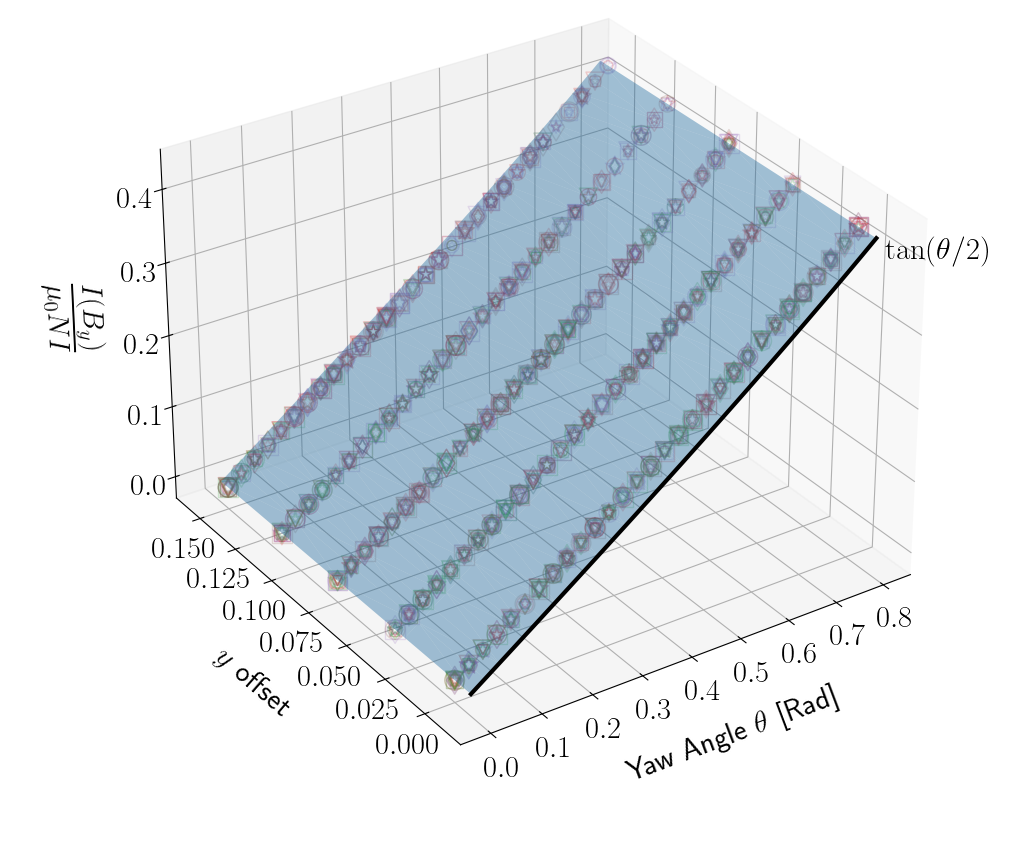
\includegraphics[width=0.8\linewidth]{figs/ByInt3D}
    \caption{Scatter plot with a random subset of simulation results.}
    \label{fig:ByInt3D}
\end{figure}



A randomly chosen subset of the simulation results are plotted in figure \ref{fig:ByInt3D}.
The markers shows the left hand side of equation \ref{eq:Byint-Error}
as calculated from the simulations and the right hand side is represented by the translucent
blue surface.
Each of the parameters \emph{L}, \emph{W} and \emph{R} are represented
by marker shape, size and color respectively. It can be seen that
equation \ref{eq:tanhalf} holds over all the simulated parameters.

The accuracy is further studied in figure \ref{fig:ByInt-Error},
showing the difference \newline
$\frac{I_{\vb{l}}(B_y)}{\mu_0NI} - \arctan(\frac{\theta}{2})$ and its upper
and lower bounds from every simulation, which
we will call the error function $E$. Although the error function
is never large in the simulated range of parameters,
it grows with the angle $\theta$.

\begin{figure}[h!]
    \centering
    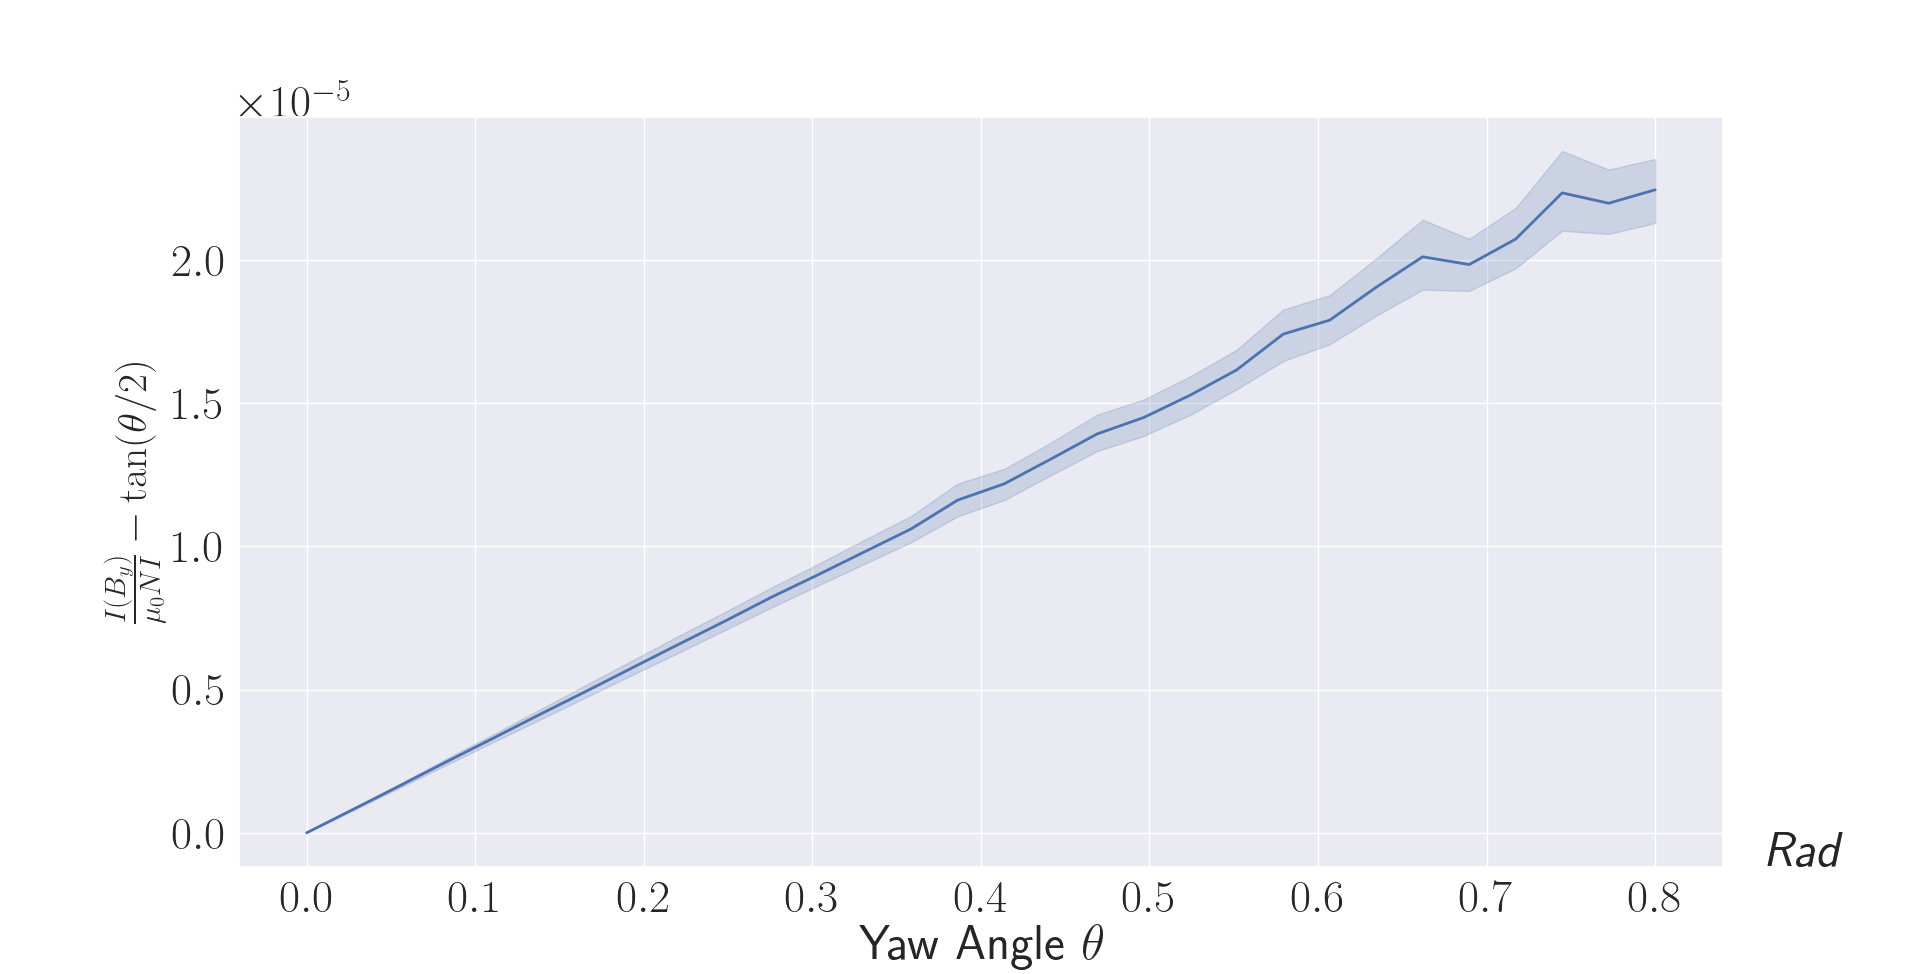
\includegraphics[width=\linewidth]{figs/ByIntError}
    \caption{Plot showing the error function $E$, comparing the simulated results
        with equation \ref{eq:Byint-Error}.}
    \label{fig:ByInt-Error}
\end{figure}


A likely cause is that as the solenoid rotates, the coil windings
get closer to the line $\vb{l}$ where the integral is evaluated. The
proximity of the singularities in the windings makes the partial derivative
of the field over $z$ higher, making the discretization errors larger.
To verify this, the error function $E$ was calculated with a single coil
model, this time varying the discretization size instead. The magnet model
used had the parameters $L=0.2$m, $W=0.05$m and $R=0.3$m. The line offset
was zero and the angle $\theta=0.8$rad.

As the number
of integration samples grows, the error shrinks up to a point where it
flattens out, as seen in figure \ref{fig:ByInt-Error-convergence}. It seems
that the limits of the numerical simulations were reached.

\begin{figure}[h!]
    \centering
    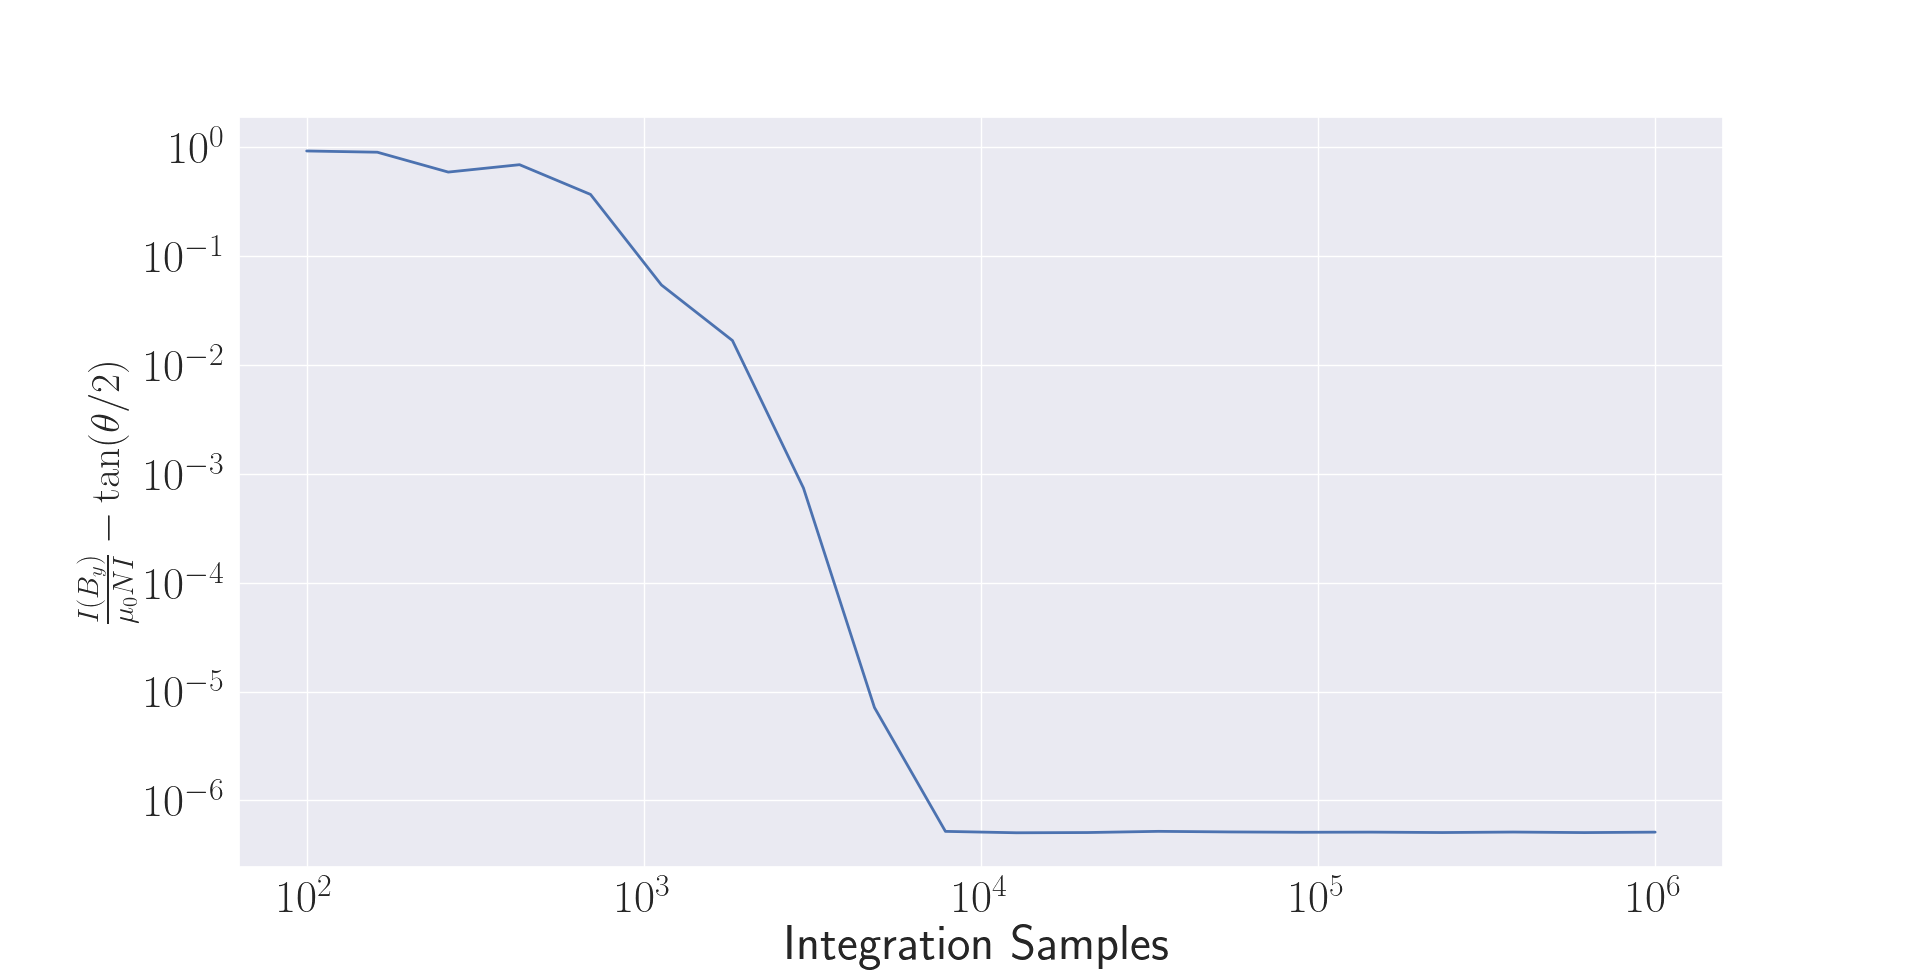
\includegraphics[width=\linewidth]{figs/ByInt-Convergence.png}
    \caption{Plot showing the error function $E$, and how it converges with
        more integration samples.}
    \label{fig:ByInt-Error-convergence}
\end{figure}

Now, looking back at the BFF series from section
\ref{subsubsection:solenoid-harmonics}, specifically the
multipoles in $r$ and $\varphi$ as in equation \ref{eq:BFFmultipoles}

\begin{equation}
    \Bffno
    \label{eq:BFFmultipoles}
\end{equation}

the simulation results presented above can be used to determine
these coefficients. All other components will vanish in the
integrals \ref{eq:By-Integral} and \ref{eq:Bx-Integral} since
$\vb{l}$ spans exactly one period. Furthermore, the
$x$ and $y$ offset do not affect the value of the integral.
This suggests that no higher order multipoles than the dipoles are
created when the solenoid is tilted, since they vary with $x$ and $y$ 
(or $r$ and $\varphi$, analogously). Using similar reasoning as
in equation \ref{eq:Czz}, the following can be said about the
dipole components in $r, \varphi$ for the BFF series

\begin{align}
    |C_{1,0} + C_{-1,0}|     & \approx \mu_0
    \tan\left( \frac{\theta}{2} \right) \frac{NI}{L}    \\
    \arg(C_{1,0} + C_{-1,0}) & = \alpha + \frac{\pi}{2}
\end{align}
where $\alpha$ is the angular offset from the $x$ axis to the rotation
axis of the solenoid.

\chapter{Results and Discussion}
To estimate the magnetic field in tesla from the flux measurements
(in webers), the signals must be deconvoluted. The most simple
such deconvolution is simply dividing the flux $\Phi$ by the total surface
area of the coil $A_{coil}$, as in equation \ref{eq:Phi-Area}
\begin{equation}
    \hat{B}[z] = \frac{\Phi[z]}{A_{coil}}
    \label{eq:Phi-Area}
\end{equation}
This gives an estimate $\hat{B}$ of the average $\vb{B}$ field
flowing through the whole coil. The area of the coil can be acquired
either by measuring a known dipole field, or estimated from the
PCB CAD drawings.

Another possibility is fitting the BFF series described in section
\ref{subsec:BFF}, which would give a full three dimensional map of
the whole measurement domain. This is more complicated however,
and requires good modeling of the PCB coils.

\section{Coil Modeling}
\label{sec:coil-modeling}
To fit the BFF series to the flux measurements from the translating
fluxmeter, one needs to take the surface integrals of the coils.
The coil shapes are made up of several spiraling turns, and cannot be
well approximated by simple geometric figures.
Furthermore, the coils span ten layers,
where they start and end at different positions at each layer to make
room for the vias connecting the tracks. Therefore, a python library
was developed to automatically estimate the surfaces from the
PCB CAD files. Each coil first needs to be converted to an
ordered polygon, an ordered set of points defining the path
of the coil.

The CAD files were first converted to KICAD format, an open source
PCB design program. Being open source, the files are easily parsed
since the format is openly available. \cite{noauthor_board_nodate}
Each coil (or net in PCB terms) is then imported, keeping metadata such as
the layer and track width. For each net, there is then an unsorted
array of all the track sections making up the net. Each track
section consists of a start point, an end point and the metadata.
For curved tracks, there is also a mid point. From the three points
a circle can be defined, where a section of the perimeter of the
circle makes up the curved track section. The curved tracks are in the
end discretized as several smaller straight tracks.

Since the tracks are unsorted, and do not necessarily have the
same direction, they need to be sorted. This is done layer by
layer. For each layer, there is an array of $n$ unordered tracks,
with start points $\vb{s_i}$ and end points $\vb{e_i}$.

\begin{equation}
    \begin{pmatrix}
        \vb{s_0} & \vb{e_0} \\
        \vb{s_1} & \vb{e_1} \\
        \vdots   & \vdots   \\
        \vb{s_n} & \vb{e_n} \\
    \end{pmatrix}
\end{equation}

The start and end points are concatenated into one
$n\times 1$ array. To make further equations more clear,
all points will be renamed $\vb{p_i}$
\begin{equation}
    \begin{split}
        &\begin{pmatrix}
            \vb{s_0} &
            \vb{s_1} &
            \cdots   &
            \vb{s_n} &
            \vb{e_0} &
            \vb{e_1} &
            \cdots   &
            \vb{e_n}
        \end{pmatrix}^T = \\
        &\begin{pmatrix}
            \vb{p_0} & \vb{p_1} & \cdots & \vb{p_{2n}}
        \end{pmatrix}^T
    \end{split}
\end{equation}

A distance matrix $M$ of size $2n\times 2n$ is then computed,
containing the pairwise distances of all points.
\begin{equation}
    M =
    \begin{pNiceMatrix}
        \pdist{0}{0}  & \pdist{0}{1}   & \Ldots     & \pdist{0}{2n}    \\
        \pdist{1}{0}  & \Ddots         &            & \Vdots           \\
        \Vdots        &                & \Ddots     & \pdist{2n-1}{2n} \\
        \pdist{2n}{0} & \Ldots         & \pdist{2n}
        {2n-1}        & \pdist{2n}{2n}
    \end{pNiceMatrix}
\end{equation}

Neighboring points are then found by extracting the boolean matrix $N$
from $M$ where the elementwise distances are smaller than some radius $r$.
$r$ is set to be equal to the track width to start, but is iteratively
decreased if the points have more neighbors than expected. This can happen
if the coils contains very short tracks. Each row of $N$ corresponds to
a point, and each column in that row that is equal to 1 corresponds to a
neighbor.

The first $n$ rows in $N$ corresponds to the track
start points, and the last $n$ rows correspond to the track end points.
Then each track segment has its start point neighbors at row $i<n$ and end
point neighbors at row $i+n$. To find the corresponding point $j$ in a track
start/end pair, one simply needs to take the modulus of the row number $i$,
as in equation \ref{eq:trackmodulus}.
\begin{equation}
    j = (i+n)\mod 2n
    \label{eq:trackmodulus}
\end{equation}

Two points on each layer has zero neighbors (excluding the diagonal in
$N$). These are the start and end
points on that layer, connected to a via or a soldering contact on the
first and last layers. Every other point has one neighbor excluding
itself.
The first one of the zero neighbor points is used as a starting point
for the algorithm. Using equation \ref{eq:trackmodulus}, the pair
point for that track segment is found. Continuing, this track segment
will have one neighbor, which is the next point in the polygon. This
continues for all points in the layer, until the other point with no
neighbors is found. For each track segment, one of the start or
end points are discarded, while the other one is put into a polygon
array. This is repeated for each layer in the PCB. The start and end
points for each layer are then matched up to find the orientation
of each polygon array. All layers are then concatenated into one
single polygon array, with the respective layer height added to
each point. The whole coil is now discretely parametrized as an
ordered set of three dimensional points. A plot of one such
set can be seen in figure \ref{fig:pcbpolygon}.

\begin{figure}[!h]
    \centering
    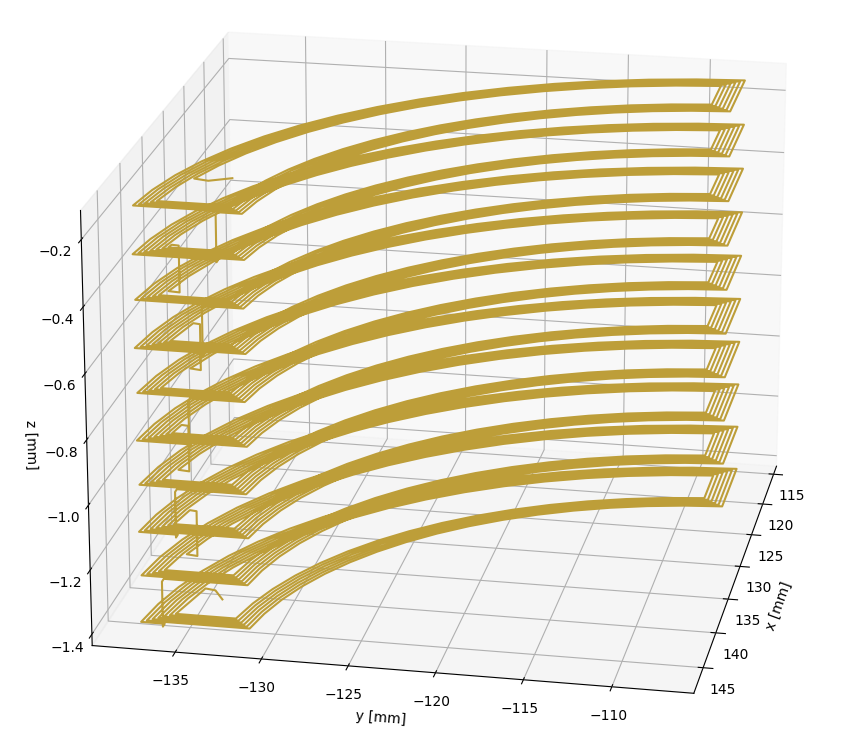
\includegraphics[width=0.8\linewidth]{figs/pcbpolygon}
    \caption{Q31 as an ordered polygon.}
    \label{fig:pcbpolygon}
\end{figure}

With the coils in this polygon format, their total surface area can easily
be approximated using for example the shoelace formula \cite{braden_surveyors_1986}.
This works as a good estimate for the area in equation \ref{eq:Phi-Area}.
For a full deconvolution however, the total surface area is not
enough. The geometric distribution of the surface is also important.

For this purpose, the coil polygons were used to make indicator
functions $\vb{1_A}$. These functions have the property that:
\begin{equation}
    \vb{1_A}(\vb{r}) = \left\{
    \begin{matrix}
        1, & \text{if } \vb{r} \in \vb{A} \\
        0, & \text{otherwise}
    \end{matrix}
    \right.
\end{equation}
where $\vb{A}$ is a surface. The magnetic flux integral of a
coil surface with indicator function $\vb{1_C}$ is then

\begin{equation}
    \Phi(\vb{r}) =
    \int\limits_{-\infty}^{\infty}\int\limits_{-\infty}^{\infty}
    \vb{B}(\vb{r})\vb{1_C}(\vb{r})d\vb{r}
\end{equation}

Several surfaces are estimated for each coil, one for each turn,
on every layer. First, a central point $p_c$ inside the coil is found.
All points on one layer of the coil polygon are converted to
polar coordinates. The central point is then found by taking
the mean of the $r$ and $\varphi$ coordinate. With the central
point found, the coil polygon
$\vb{P} = \left(\vb{p_1}, \vb{p_2} \cdots \vb{p_n} \right)$
is then split into several whole turns using algorithm
\ref{alg:turnsplit}.

\begin{algorithm}
    \caption{Turn-split algorithm for pcb wound coils.}
    \label{alg:turnsplit}
    \begin{algorithmic}
        \State TurnIndices = List()
        \State Turns = 0
        \State angle = 0
        \For{$\vb{p_i} = \left(\vb{p_1}, \vb{p_2} \cdots \vb{p_{n-1}}
                \right)$}
        \State $\vb{v_1} = \vb{p_c} - \vb{p_i}$
        \State $\vb{v_2} = \vb{p_c} - \vb{p_{i+1}}$
        \State angle $+= \vb{v_1}\cdot\vb{v_2}
            /(\|\vb{v_1}\|\|\vb{v_2}\|)$
        \If{angle $>= $Turns$\cdot2\pi$}
        \State \textbf{Append} i to TurnIndices
        \State Turns $+= 1$
        \EndIf
        \EndFor
    \end{algorithmic}
\end{algorithm}

Essentially, for every point in the coil polygon, two vectors
are drawn from the central point to the current and next point
in $P$. The angle $\varphi$ between these vectors is calculated using their
inner product. This is repeated until the cumulative angle is more
than $2\pi$ times the currently reached number of turns. The indice
of every full turn is saved to a list. This algorithm is also illustrated
in figure \ref{fig:Q11-winding}.

\begin{figure}[!h]
    \centering
    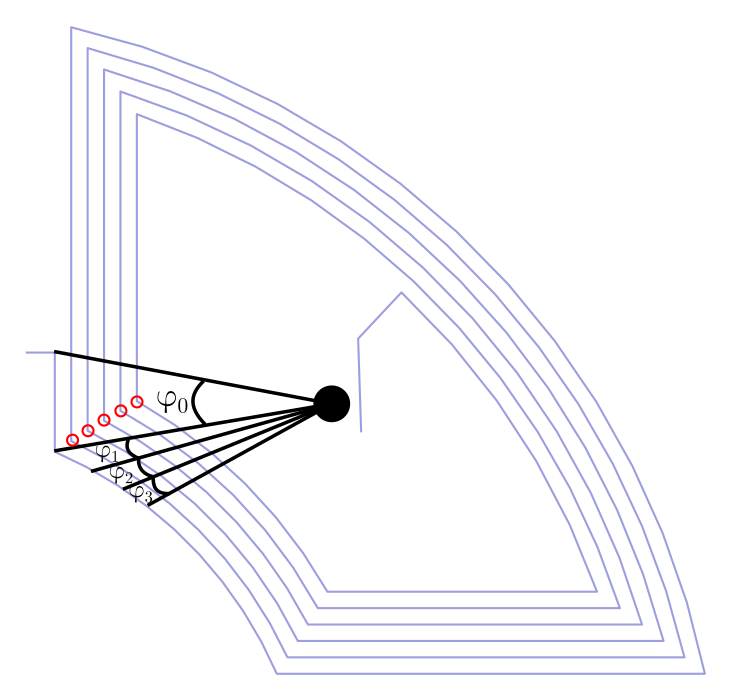
\includegraphics[width=0.8\linewidth]{figs/Q11-roundwalk}
    \caption{Q11 coil winding, with the central point, some
        partial angles, and the estimated start/end points of
        the turns in red.
        Note that curved segments are discretized into smaller
        straight segments.}
    \label{fig:Q11-winding}
\end{figure}

Once the indices for all turns have been found, the polygon is
split into several polygons, one for each turn. The turn polygons
are closed by making them start and end at the same point. Each
coil now has a total amount of turns times layers polygon surfaces.
Two such surfaces can be seen in figure \ref{fig:coilsurfaces}.
In practice, every turn surface is the union of all that turns
surfaces across the layers, to save on expensive surface
integral computations. This slightly
overestimates the amount of surface, but also "smooths" over
the irregularities from the vias and irregular start/end points
across the layers. The surface integrals then only need to
computed once for each turn, and then the results multiplied
by the number of layers.

\begin{figure}[!h]
    \centering
    \begin{subfigure}[b]{0.4\textwidth}
        \centering
        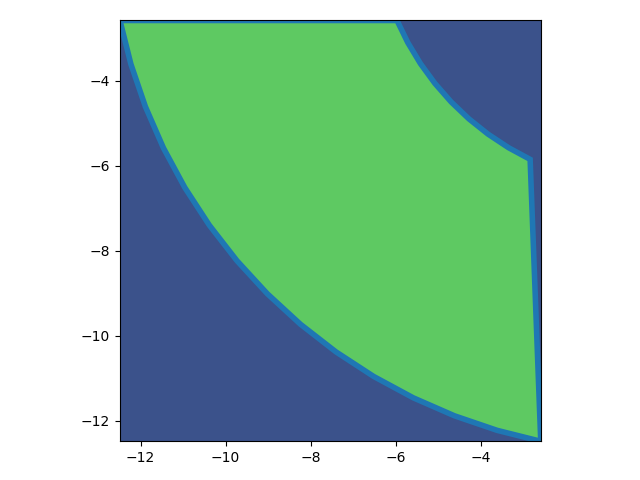
\includegraphics[height=100pt]{figs/Q11-layer0}
        \caption{$Q_{3,1}$ outermost turn surface estimation.}
    \end{subfigure}
    \hfill
    \begin{subfigure}[b]{0.4\textwidth}
        \centering
        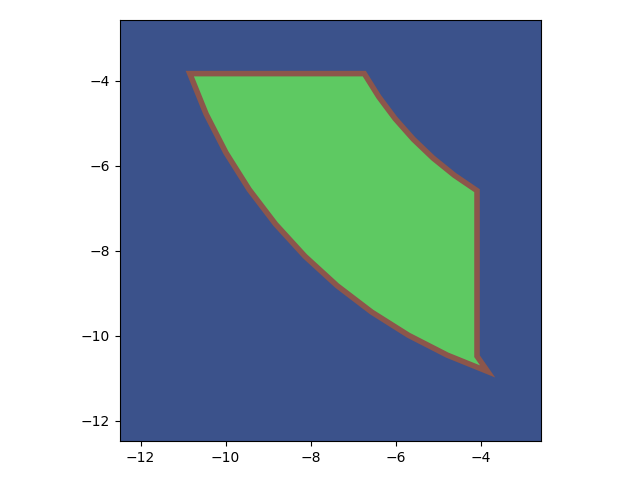
\includegraphics[height=100pt]{figs/Q11-layer5}
        \caption{$Q_{3,1}$ innermost turn surface estimation.}
    \end{subfigure}
    \caption{Estimated coil surface polygons.}
    \label{fig:coilsurfaces}
\end{figure}

The PCB coils have 10 layers with 7 turns per layer. Thus, every
coil produces 7 indicator functions, one for every turn.


\section{Coil Deconvolution and Sensitivity}
\label{sec:coil-deconvolution}
With a way to compute the flux integrals of the coils, the
magnetic flux density can now be properly deconvoluted
from the flux measurements. The flux integral for a
coil can be rewritten in terms of the BFF series.
Since the coils are translated through the magnet
with their normal vector parallel to the $z$ axis, the estimated
flux integral $\hat{\Phi}_C$
for a coil $C$ with surface $A_C$ becomes

\begin{equation}
    \begin{split}
        \hat{\Phi}_C[z_i] &=
        \iint\limits_{A_C}
        \sum\limits_{n=-\infty}^{\infty}
        \sum\limits_{k=-\infty}^{\infty}
        \frac{\partial \Psi_{n,k}}{\partial z}
        (r,\varphi, z|z=z_i) dA \\
        &= \sum\limits_{n=-\infty}^{\infty}
        \sum\limits_{k=-\infty}^{\infty}
        \iint\limits_{A_C}
        \frac{\partial \Psi_{n,k}}{\partial z}
        (r,\varphi, z|z=z_i)dA
    \end{split}
\end{equation}

Let $\psi_{n,k} = \Psi_{n,k}/\Cnk[n,k]$. Since $\Cnk[n,k]$ are
constants, they can be moved out of the integral.

\begin{equation}
    \hat{\Phi}_C[z_i]
    = \sum\limits_{n=-\infty}^{\infty}
    \sum\limits_{k=-\infty}^{\infty}
    \Cnk
    \iint\limits_{A_C}
    \frac{\partial \psi_{n,k}}{\partial z}
    (r,\varphi, z|z=z_i)dA
    \label{eq:psi-integral}
\end{equation}

Let $|n| < N, |k| < K$.
Equation \ref{eq:psi-integral} can now be
written as a matrix equation

\begin{equation}
    \begin{split}
        &\hat{\Phi}_C[z_i] = \\
        &=\iint\limits_{A_C}
        \frac{\partial}{\partial z}
        (\psi_{-N, -K}, \psi_{-N, -K+1}, \ldots,
        \psi_{0, 0}, \ldots, \psi_{N, K-1}, \psi_{N, K})
        dA
        \begin{pmatrix}
            \Cnk[-N, -K] \\ \Cnk[-N, -K+1]\\ \vdots\\
            \Cnk[0, 0]   \\ \vdots \\ \Cnk[N, K-1]\\ \Cnk[N, K]
        \end{pmatrix}
    \end{split}
\end{equation}

Now, denote the leftmost column vector as $\vb{V}_C[z_i]$,
containing the terms of the surface integrals of $\psi_{n,k}$,
with integral surface of coil $C$ at $z$ offset $z_i$. The flux
measurements can now be inserted into the matrix equation, denoting
a measurement sample from coil $C$ at position $z_i$ with $s_C[z_i]$.
This allows us to formulate the measurements and BFF series as
a least squares problem. Let $X$ be the matrix of surface
integrals, $\frak{C}$ the row vector of $\Cnk$ coefficients,
$E$ the row vector of measurement and modeling errors $e[z_i]$, and
$S$ the row vector of measurement samples. The model is then
formulated as $X\frak{C} + E = S$, or more explicitly written
in equation \ref{eq:matrixmodel}.


\begin{equation}
    \begin{pmatrix}
        \vb{V}_C[z_0]     \\ \vb{V}_C[z_{1}] \\ \vdots \\
        \vb{V}_C[z_{i-1}] \\ \vb{V}_C[z_i]
    \end{pmatrix}
    \begin{pmatrix}
        \Cnk[-N, -K] \\ \Cnk[-N, -K+1]\\ \vdots\\
        \Cnk[0, 0]   \\ \vdots \\ \Cnk[N, K-1]\\ \Cnk[N, K]
    \end{pmatrix}
    + \begin{pmatrix}
        e[z_0]     \\ e[z_1]\\ \vdots\\
        e[z_{i-1}] \\ e[z_i]
    \end{pmatrix} =
    \begin{pmatrix}
        s_C[z_0] \\ s_C[z_1] \\ \vdots \\ s_C[z_{i-1}] \\
        s_C[z_i]
    \end{pmatrix}
    \label{eq:matrixmodel}
\end{equation}

The least squares problem is then formulated as finding the
coefficients $\frak{C}$ that minimizes the expression
$\| X\frak{C} - S \|$.
The $\Cnk$ coefficients can now easily be found using a
least squares solver. Furthermore, measurements from
several coils can be added to the equation, allowing one
to fit one model to as many coils as desired.

The $X$ matrix is of particular interest. It contains the
surface integrals of all given coils. This gives a good
indication of the sensitivity of the coils to the different
harmonics in the BFF series. This matrix is visualized in
figure \ref{fig:sensitivity}. Only the coils with unique
geometries are visualized. $Q_{1,4}$ and $Q_{2,4}$ will
for instance have the exact same sensitivity since they
are geometrically identical, save for their rotation and
position on the coil.

\begin{figure}[!h]
    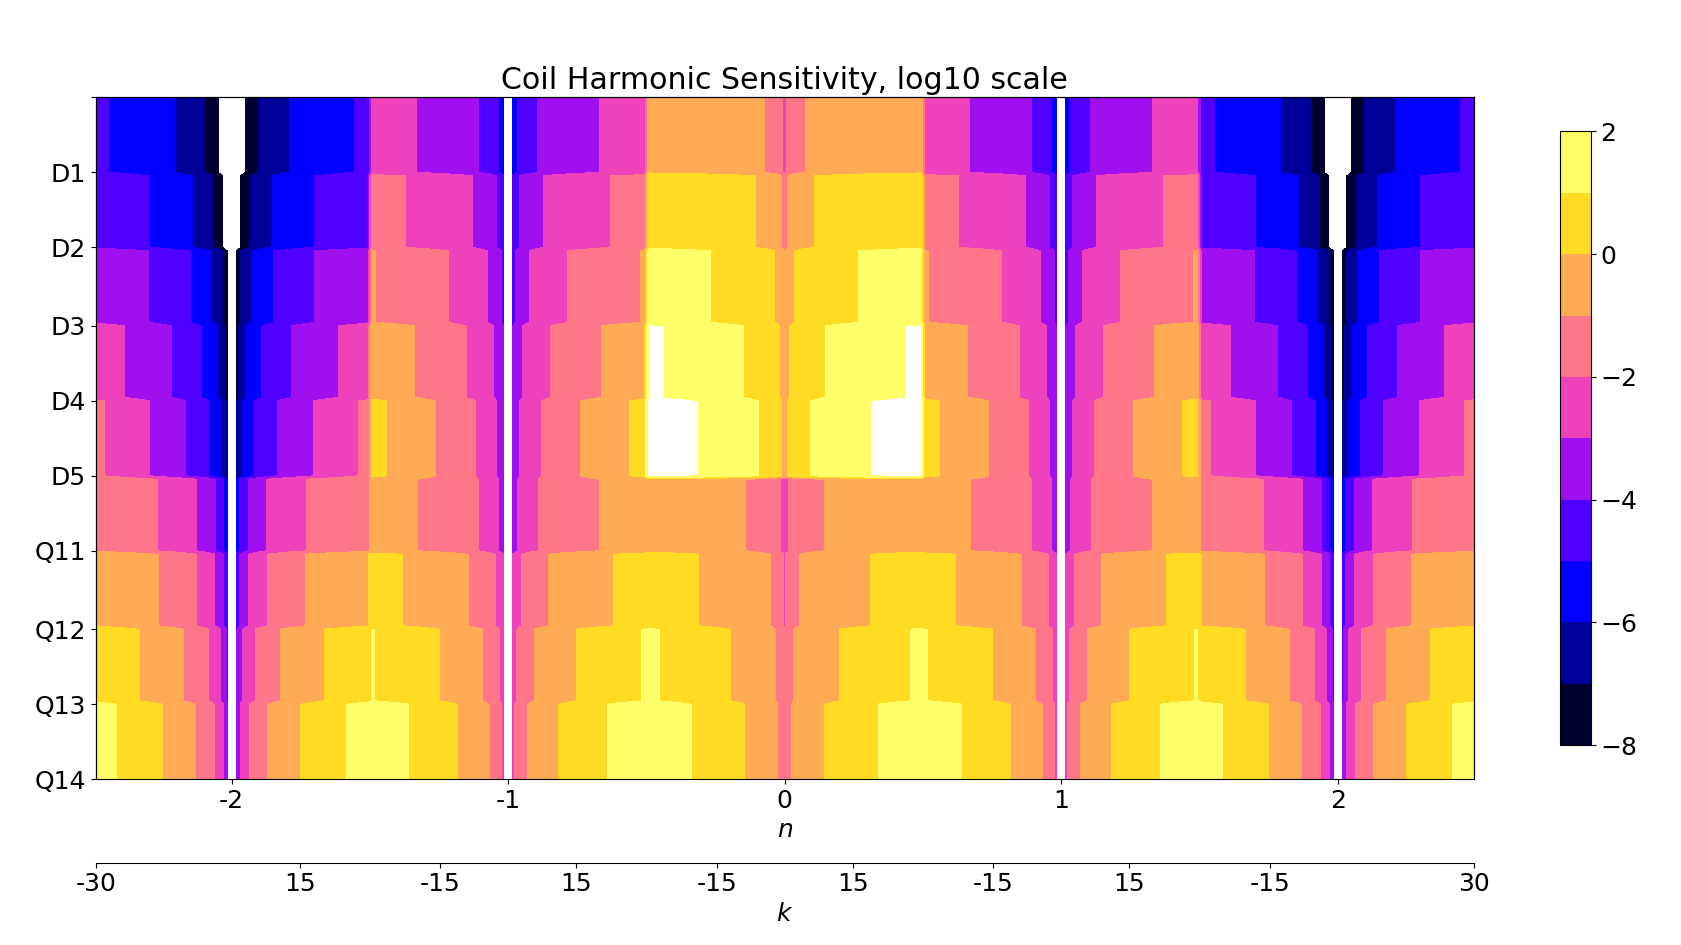
\includegraphics[width=\linewidth]{figs/sensitivity}
    \caption{Sensitivity for the different coils present on
        the fluxmeter.}
    \label{fig:sensitivity}
\end{figure}

Some interesting (and mostly expected) conclusions can be drawn
from figure \ref{fig:sensitivity}. The disc coils are
several orders of magnitude more sensitive to the
solenoid fundamentals than the harmonics, verifying that
they're insensitive to the peak shift from magnet tilt, as
seen in the measurements. The sector coil are on the other
hand relatively much more sensitive to higher orders of both $k$
and $n$, making them a lot more sensitive to the peak shifts.
The disc coils, particularly the largest ones have the largest
sensitivity to any single component, simply because they have more
surface area.
No coils are sensitive to the multipole components. Because
the $B_r$ and $B_\varphi$ components vanish in the flux integrals,
so do the multipole components. This is unfortunate, as it means
that only the $B_z$ field can be fully estimated using this model.

It should be noted that the coil sensitivity is not the only thing
predicting a good fit. One must be mindful of the Nyquist criterium
in all three dimensions. The Bessel-Fourier-Fourier series is
a fourier series in $\varphi$. Therefore, the number of coils
spread out over $\varphi$ puts an upper bound on $n$.
Likewise, the number of samples
along the $z$ axis puts an upper bound on the order of $k$. From
equation \ref{eq:Psi} it can be seen that the geometric frequency
in $z$ $f_z$ can be expressed as
\begin{equation}
    f_z = \frac{2\pi}{L}|k|
    \label{eq:fz}
\end{equation}
and the geometric frequency in $\varphi$
\begin{equation}
    f_{\varphi} = |n|
    \label{eq:fphi}
\end{equation}

\section{Bessel-Fourier-Fourier Series Fitting}
\label{sec:BFF-fitting}
On the fluxmeter, there are four
sector coils per radial layer, giving us four points in $\varphi$.
Using the Nyquist criterion along with equation \ref{eq:fphi}
then gives us the upper bound on fitting in $n$
\begin{equation}
    |n|_{\text{max}} < \frac{4}{2} = 2
\end{equation}

The maximum order of $k$ can be computed in a similar way
using equation \ref{eq:fz}.
The measurements are spaced
along the z axis with a distance of $0.11$ mm, or
$\frac{1}{0.00011} \approx 9090$ samples/m. The fluxmeter
measurements spanned 1.5 meters.
The upper bound on $k$ can then be found
\begin{equation}
    |k|_{\text{max}} < \frac{9090\cdot 1.5}{2\cdot 2\pi} \approx 1085
\end{equation}
When fitting in practice, an order $k=30$ was found to be
more than sufficient for a good fit, and $n$ was chosen to
be equal to 1. Through experimentation, it was also found
that fitting using just the $D_5$ coil and the outermost
sector coils $Q_{1,4}-Q_{4,4}$ was sufficient. A better fit
was not achieved by using more coils. By studying figure
\ref{fig:sensitivity}, one can see that the measurements
from these coils is enough to determine the $\Cnk$
coefficients, or at least that the remaining coils give
little further benefit to the fit. In this section, a
fit of a measurement with a yaw angle of $58$ mrad is
showcased.

The fits are plotted along with their respective measurements
in figures \ref{fig:Dfit}-\ref{fig:Q1fit}. The errors for
some chosen coils can be seen in table \ref{tab:fitting-errors}.

From these results, it can be seen that the
fitting error is generally around the same magnitude, but tends
to be smaller the larger the coil is, both in absolute and
normalized terms. A likely explanation is that for coils
with a smaller surface area, errors in the coil surface
modeling will have a larger impact.

\begin{table}[!h]
    \centering
    \begin{tabular}{l p{2cm} p{2cm} p{2cm} p{2cm}}
            & Mean Error {[}Wb{]} & Max Error {[}Wb{]} & Mean Error Normalized & Max Error Normalized \\ \hline
        D1  & 1.30E-05            & 3.50E-05           & 3.08\%                & 8.30\%               \\
        D2  & 2.07E-05            & 4.17E-05           & 0.73\%                & 1.48\%               \\
        D3  & 1.13E-05            & 2.36E-05           & 0.13\%                & 0.28\%               \\
        D4  & 4.18E-05            & 8.63E-05           & 0.24\%                & 0.50\%               \\
        D5  & 4.84E-06            & 2.93E-05           & 0.02\%                & 0.10\%               \\
        Q11 & 1.08E-05            & 2.57E-05           & 4.98\%                & 11.86\%              \\
        Q12 & 7.26E-06            & 1.48E-05           & 1.23\%                & 2.50\%               \\
        Q13 & 1.61E-06            & 7.56E-06           & 0.17\%                & 0.79\%               \\
        Q14 & 1.39E-06            & 4.30E-06           & 0.10\%                & 0.32\%
    \end{tabular}
    \caption{Fitting errors for selected coils.}
    \label{tab:fitting-errors}
\end{table}

\begin{figure}[!h]
    \centering
    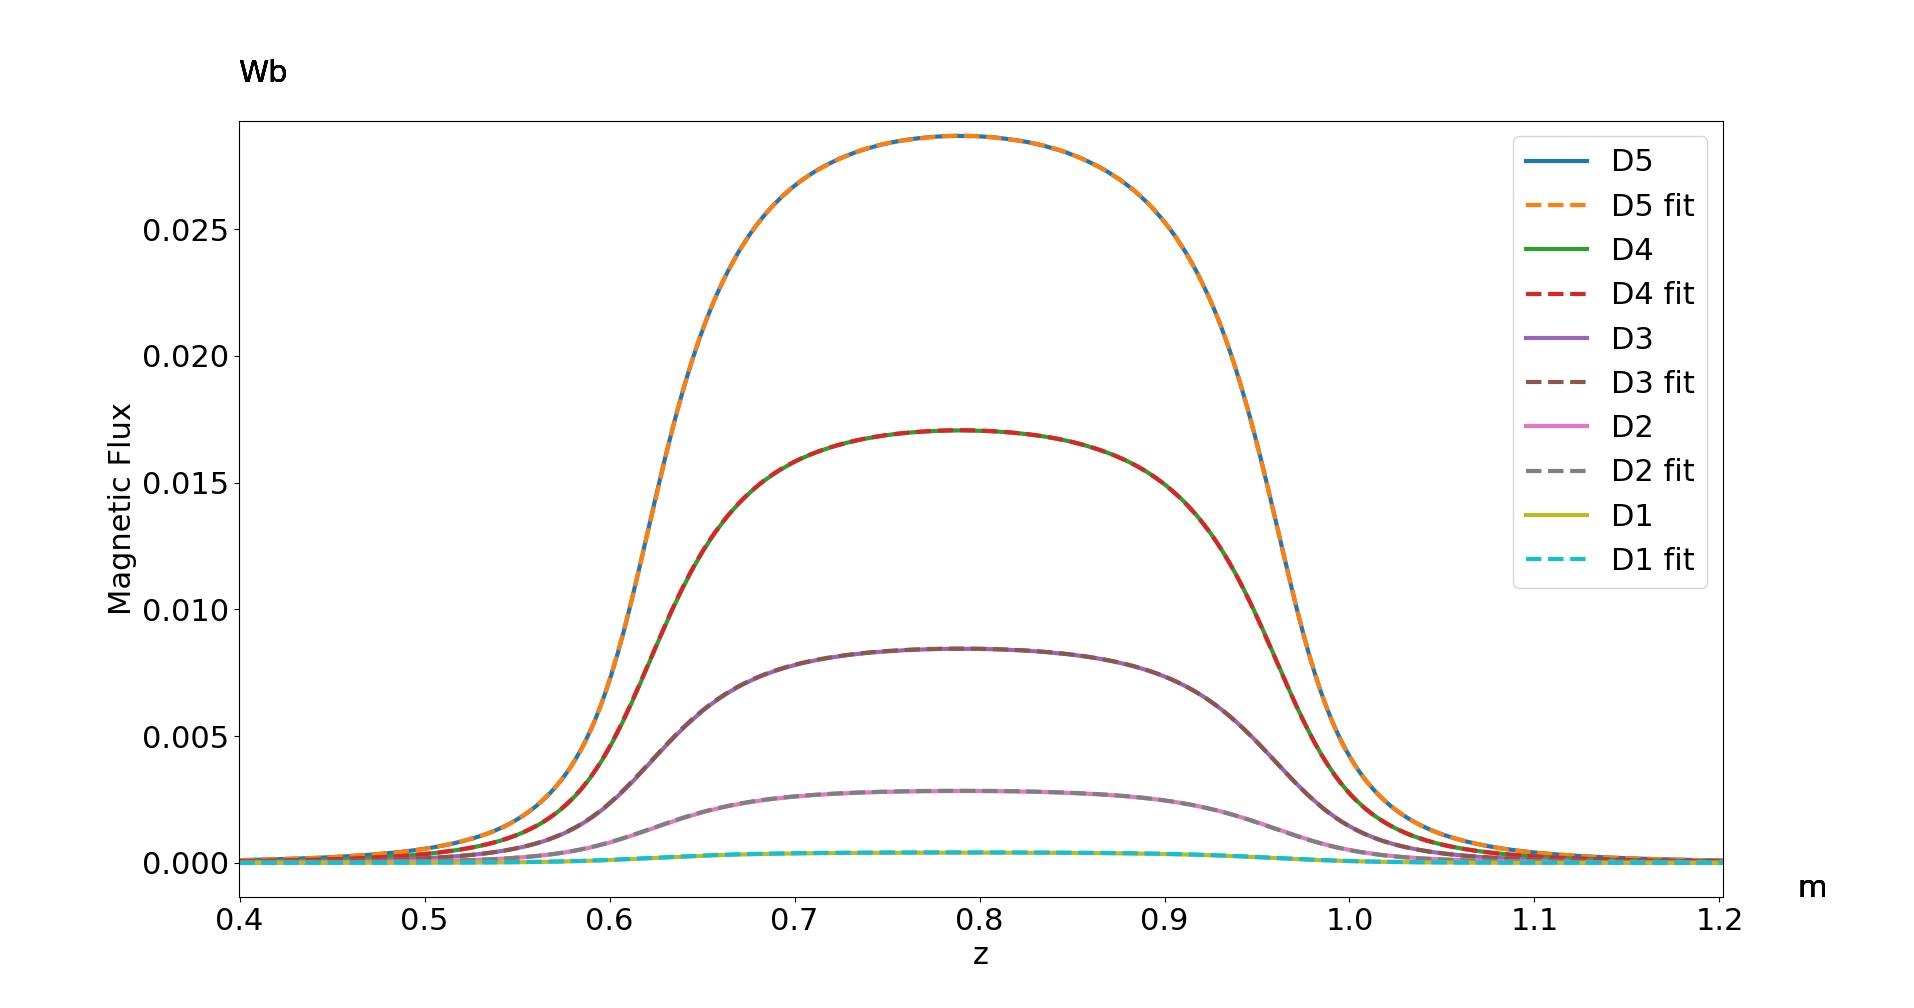
\includegraphics[width=\linewidth]{figs/Dfit}
    \caption{Measurements and BFF fit, $D_l$ coils.}
    \label{fig:Dfit}
\end{figure}

\begin{figure}[!h]
    \centering
    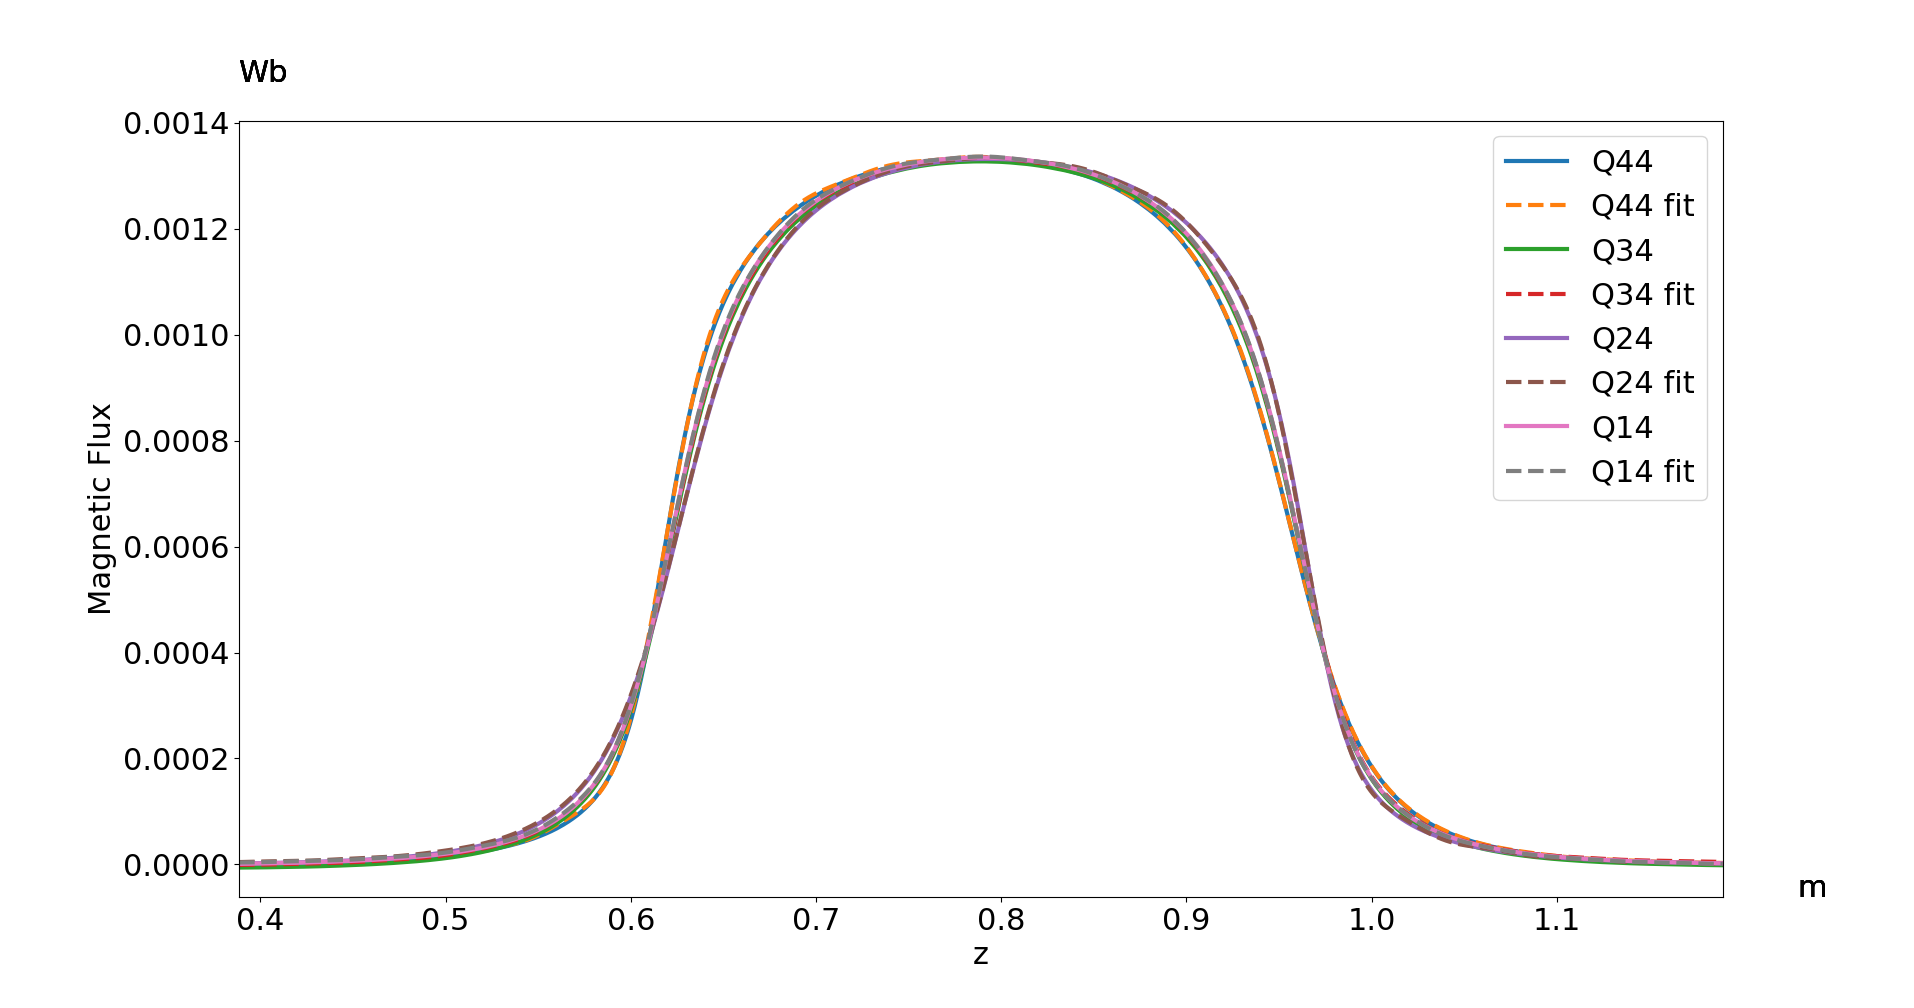
\includegraphics[width=\linewidth]{figs/Q4fit}
    \caption{Measurements and BFF fit, $Q_{q,4}$ coils.}
    \label{fig:Q4fit}
\end{figure}

\begin{figure}[!h]
    \centering
    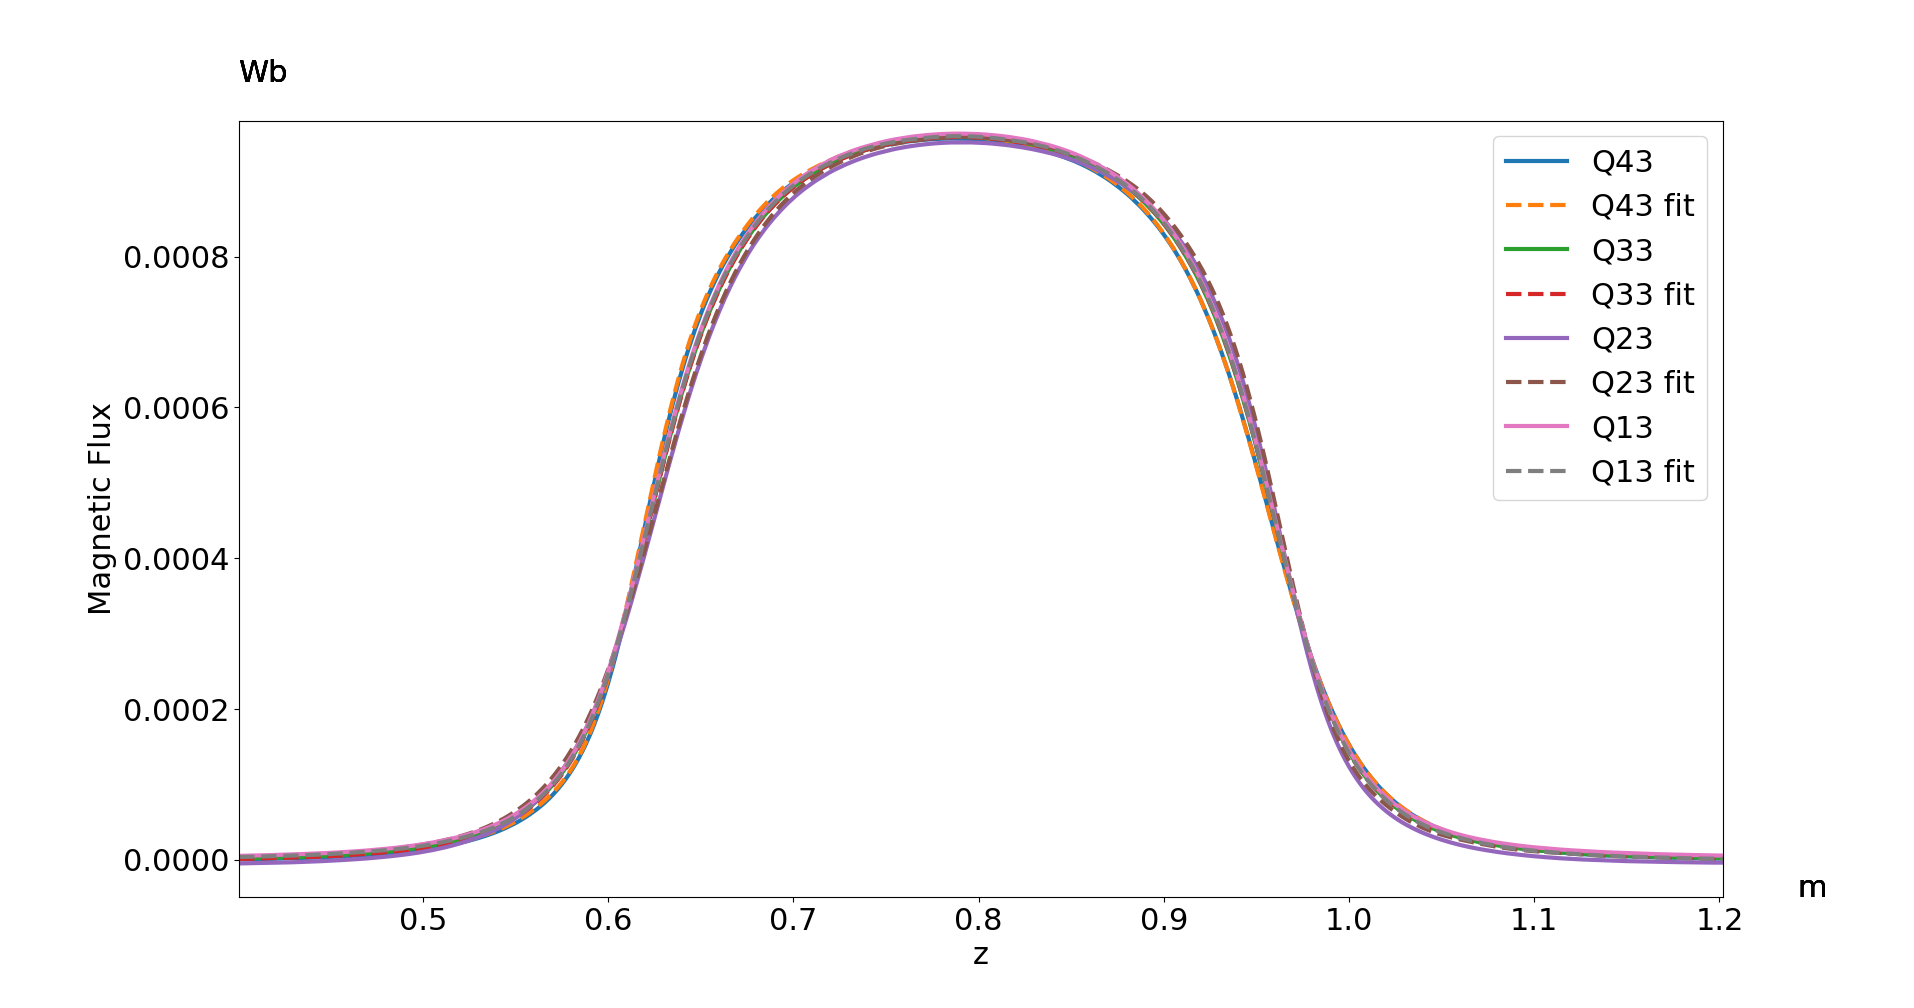
\includegraphics[width=\linewidth]{figs/Q3fit}
    \caption{Measurements and BFF fit, $Q_{q,3}$ coils.}
    \label{fig:Q3fit}
\end{figure}

\begin{figure}[!h]
    \centering
    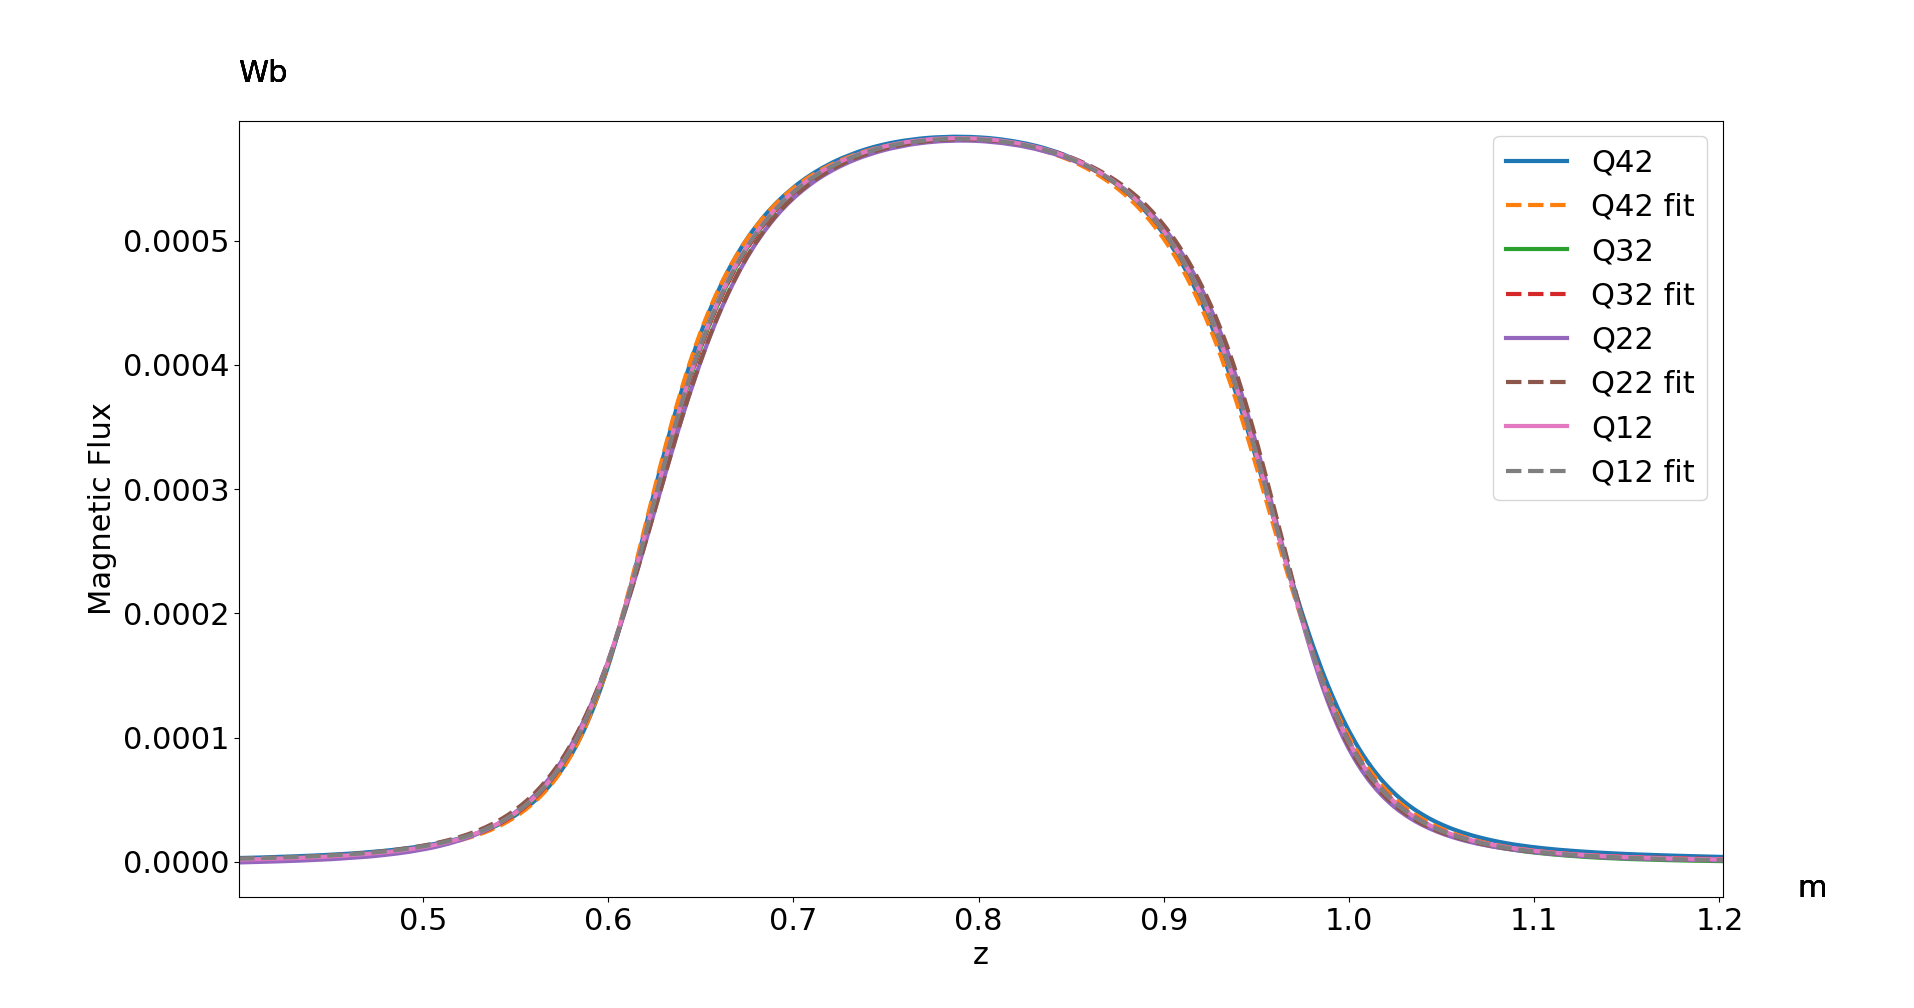
\includegraphics[width=\linewidth]{figs/Q2fit}
    \caption{Measurements and BFF fit, $Q_{q,2}$ coils.}
    \label{fig:Q2fit}
\end{figure}

\begin{figure}[!h]
    \centering
    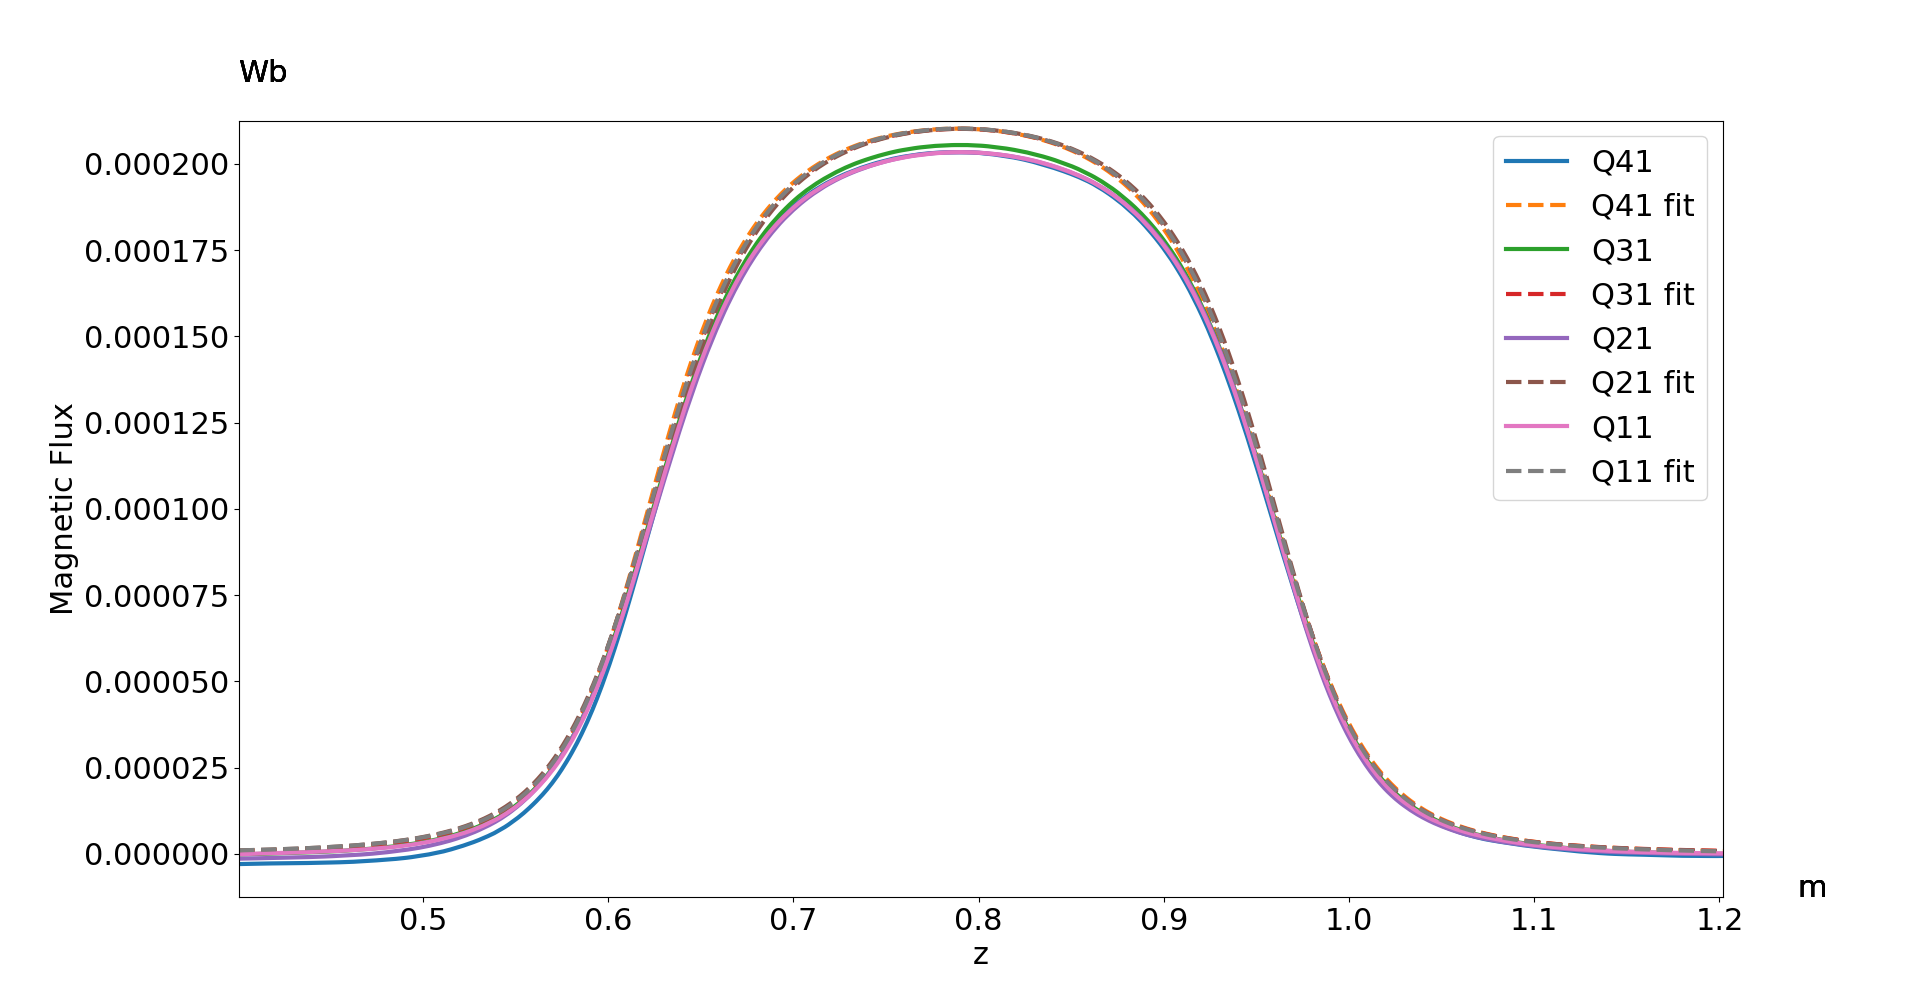
\includegraphics[width=\linewidth]{figs/Q1fit}
    \caption{Measurements and BFF fit, $Q_{q,1}$ coils.}
    \label{fig:Q1fit}
\end{figure}

\section{3D Field Maps}
With the measurements fitted, the now known $C_{n,k}$
coefficients can be used to estimate the $B_z$ field
anywhere inside the measurement domain. Some 3D maps
are presented in figures \ref{fig:3dmap}-\ref{fig:3dmapyz}

\begin{figure}[!h]
    \centering
    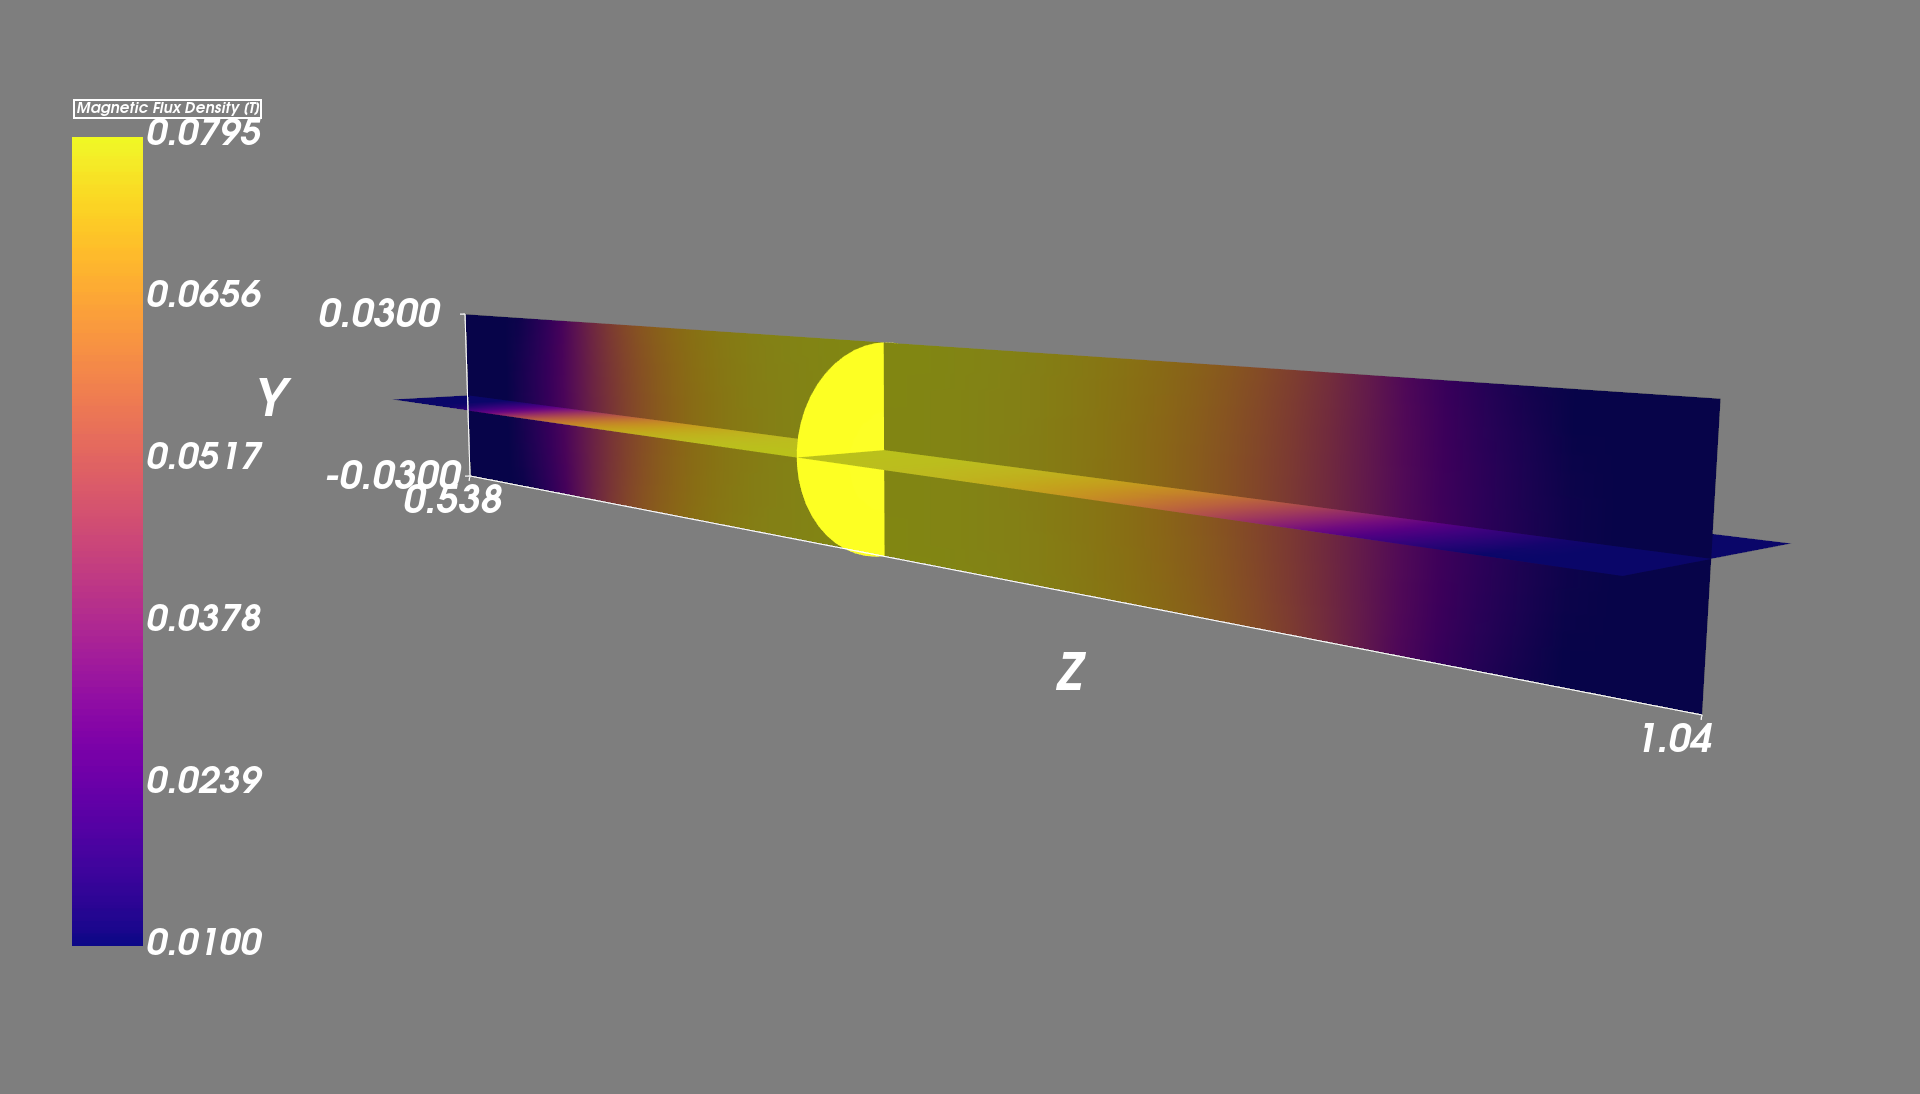
\includegraphics[width=\linewidth]{figs/3ddomain}
    \caption{3D field map of the estimated $B_z$ field.}
    \label{fig:3dmap}
\end{figure}

\begin{figure}[!h]
    \centering
    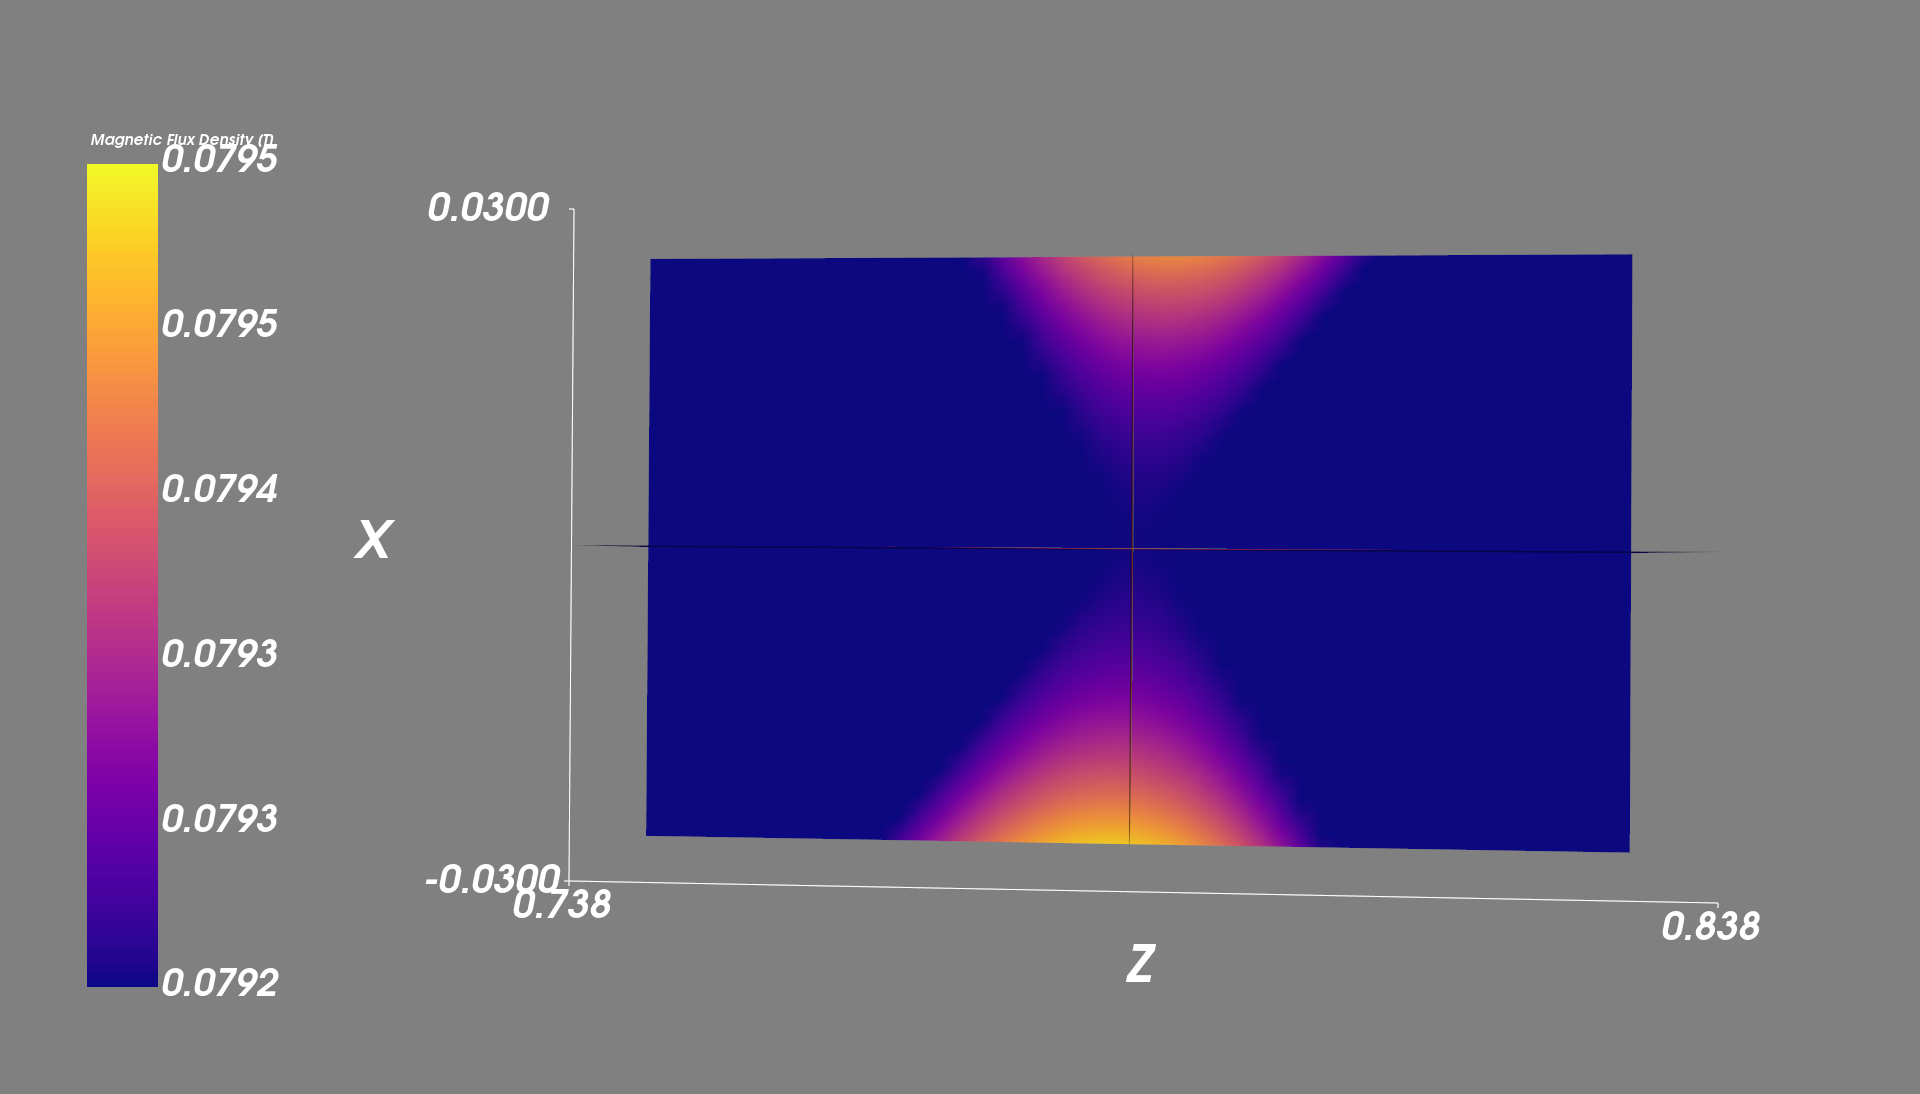
\includegraphics[width=\linewidth]{figs/3dxview}
    \caption{3D field map of the estimated $B_z$ field.
        $xz$ plane.}
    \label{fig:3dmapxz}
\end{figure}

\begin{figure}[!h]
    \centering
    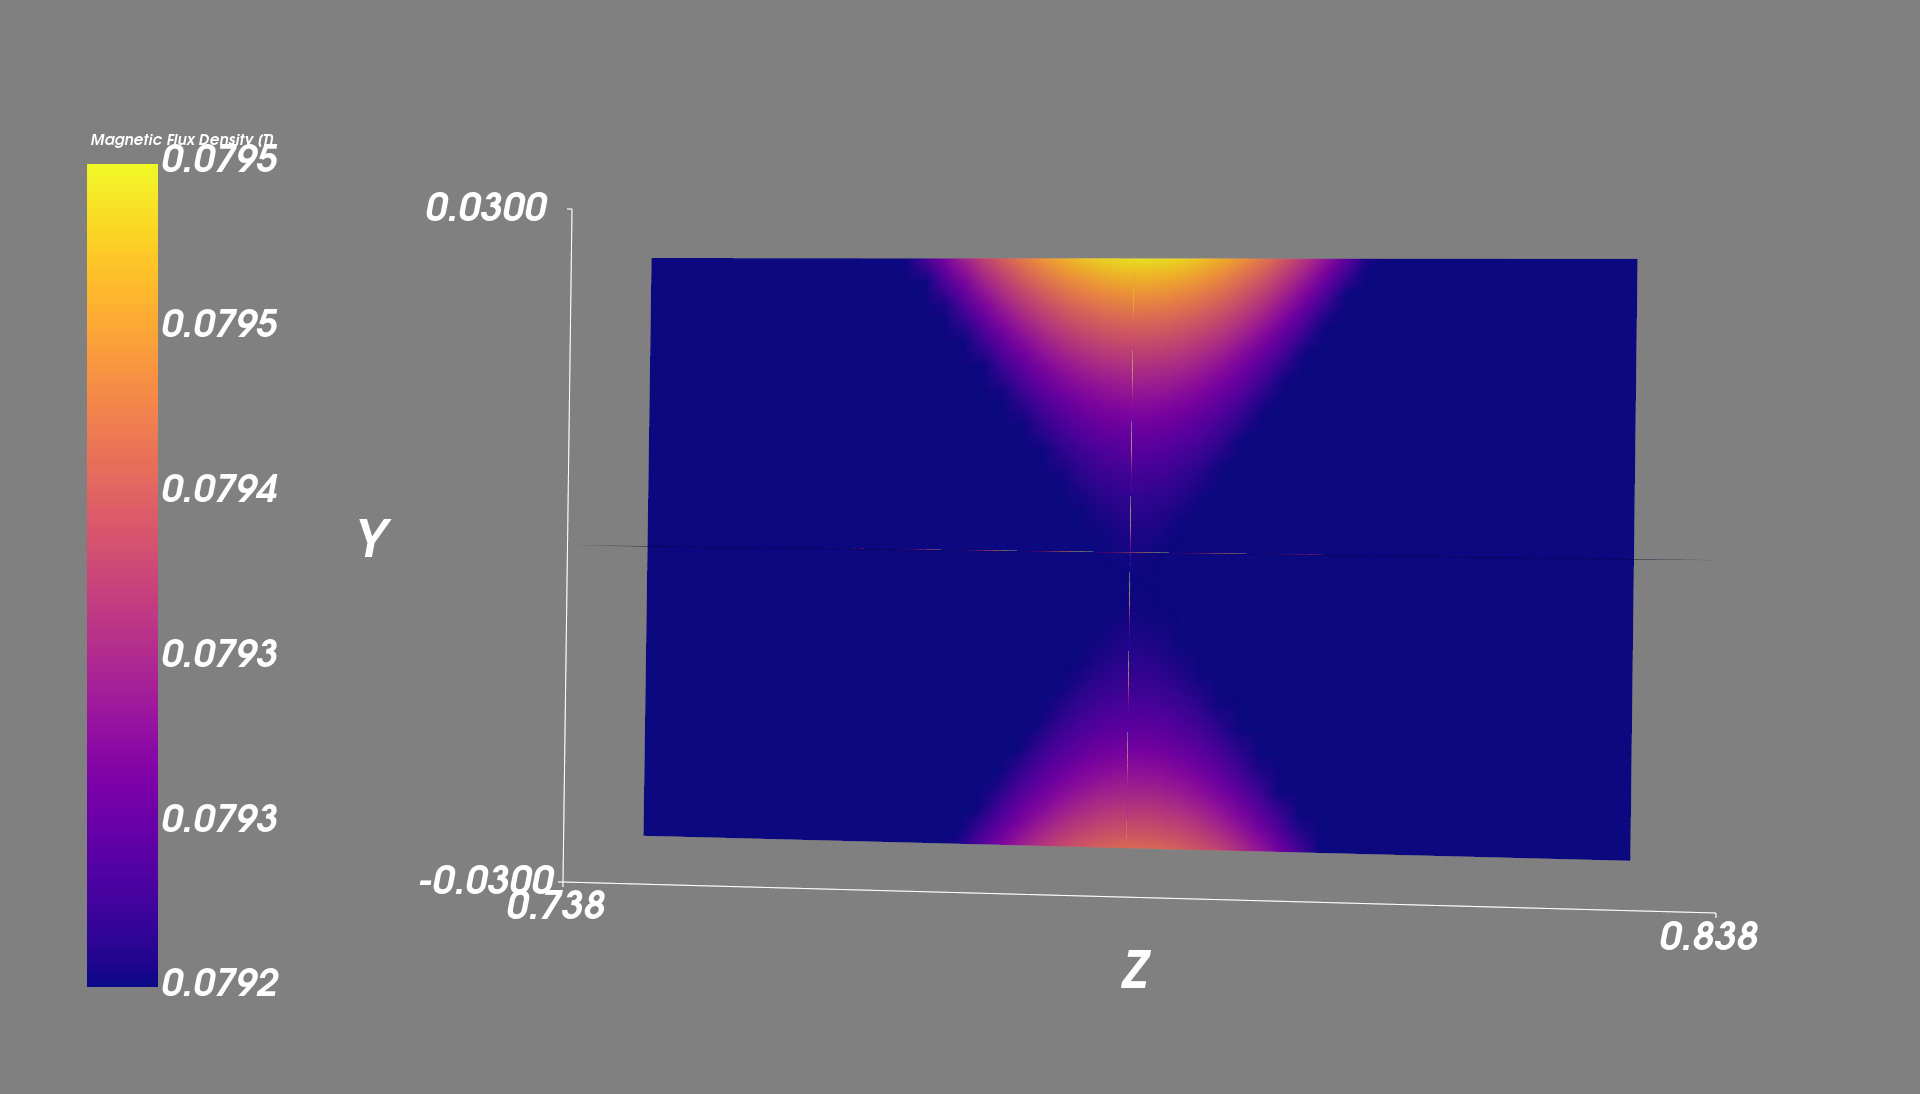
\includegraphics[width=\linewidth]{figs/3dyview.png}
    \caption{3D field map of the estimated $B_z$ field.
        $yz$ plane.}
    \label{fig:3dmapyz}
\end{figure}
\chapter{Discussion}
The angle estimation from the peak shifts turned out to be 
a harder problem than expected. As the arguments of the maximums of the
$B_z$ field is not easily modeled with regards to the offset, finding
a consistent model is a challenge. Some hope remains however. In figure
\ref{fig:sim-mag-fieldmap-argmax} one can see that the argmax tends to
the magnet ends for offsets further out. One could then build a model
taking the magnet length and aperture radius into consideration, and measure
the field as far from the center of the aperture as possible.

Another possibility is to add coils or Hall effect sensors that measure
the transversal $B_x$ and $B_y$ components. If the results of section 
\ref{sec:dipole-simulations} hold for real and not only simulated magnets,
this could be a very robust way of measuring the tilt-swing angle of the
solenoid. Although the transversal dipole moments are not as strong as
the $B_z$ field, the integral of the translating measurements is very
resistant to gaussian noise. This coupled with the fact the dipole
integral is invariant to potential offset alignment errors makes for
a promising measurement methodology.

One particularly interesting result with regards to the fitting
of the BFF series is that only the outermost coils measurements
were needed for a good fit. The innermost coils did not add any
more information. This fits well with the theory on partial
differential equations. A PDE may be completely determined
by its values at its boundaries. This also adds robustness to the system,
since the weaker field in the middle of the aperture can be estimated
using measurements of the stronger field closer to the solenoid edge,
from the more sensitive outer coils.
\clearpage


\backmatter
% References
% No restriction is set to the reference styles
% Save your references in References.bib
\nocite{*} % Remove this for your own citations
\printglossary[type=main]
\printglossary[type=unit]
%\bibliographystyle{plain}
%\bibliography{References}
\printbibliography
\end{document}